\documentclass[11pt]{article}

% FONT %

\usepackage[utf8]{inputenc}
\usepackage[T1]{fontenc}
\usepackage[italian]{babel}
\usepackage{lmodern}

% IMMAGINI %

\usepackage{graphicx}
\usepackage{float}

% MATH % 

\usepackage{amsmath}
\usepackage{amsfonts}

% ARRAY %

\renewcommand\arraystretch{1.25}

% COLORI %

\usepackage[usenames,dvipsnames,svgnames,table]{xcolor}

\definecolor{mygreen}{rgb}{0,0.6,0}
\definecolor{mygray}{rgb}{0.5,0.5,0.5}
\definecolor{mymauve}{rgb}{0.58,0,0.82}

% LINK %

\usepackage{url}
\usepackage{breakurl}
\usepackage{hyperref}
\hypersetup{
    colorlinks=true, % false: boxed links; true: colored links
    citecolor=black,
    filecolor=black,
    linkcolor=black, % color of internal links
    urlcolor=Maroon  % color of external links
}

\author{\textbf{Autore:} Federico Z. \\ \textbf{Editore Latex:} Riccardo A. \\\\Aggiornate all'AA 2019/2020}
\title{\textbf{Domande e risposte di Reti e Sicurezza}}

\begin{document}

\maketitle
\vspace{4cm}
\section*{Premesse}
Date le 73 domande che generalmente girano per l'esame di reti, mi sono permesso di reinterpretarle in maniera personale rispetto a quelle già presenti online, dando possibili risposte prendendo informazioni dal libro "Computer Networks 4th Edition" di Andrew S. Tanenbaum, unite a ricerche sul web e conoscenze personali. NON assicuro la correttezza delle risposte che NON vogliono neppure essere un riassunto al libro, vogliono servire come spunto e ripasso in preparazione dell'esame. Scià belli. \\
Federico Z. \\
\vspace{1cm} \\
Link alla repository GitHub: \url{https://github.com/FedeBrichi/Reti}

\newpage
\tableofcontents
\newpage

\section{Cosa si intende per serie di Fourier?}
Un segnale che ha una durata finita può essere gestito immaginando semplicemente che esso ripeta infinite volte l’intero schema (intervallo T e 2T è identico all’intervallo 0 a T).

È possibile quindi rappresentare i segnali tramite funzioni, le quali permettono un’analisi e una modellazione più efficace.
La Serie di Fourier non è altro che la scomposizione di un segnale in componenti sinusoidali (possibilmente infiniti).
\begin{center}
$g(t)=\frac{1}{2}c+\sum_{n=1}^\infty a_n sen(2\pi nft)+\sum_{n=1}^\infty b_n cos(2\pi nft)$ 
\end{center}

$f=1/T$ rappresenta la frequenza fondamentale, $a_n$  $b_n$  sono rispettivamente le ampiezze seno e coseno dell’n-esima armonica e \textit{c} rappresenta una costante.

Su questo teorema si basano le reti e il passaggio dei dati tramite i mezzi di trasmissione; purtroppo nella pratica i mezzi di trasmissione attenuano in modo non uniforme i componenti della serie di Fourier, generando così una distorsione. Per ovviare a questa distorsione, le ampiezze fino ad una certa frequenza vengono trasmesse senza modifiche, da quella frequenza in poi vengono attenuate.

L’intervallo di frequenze trasmesse senza una forte attenuazione è chiamato Banda Passante.
Generalmente nella realtà viene indicata la banda passante compresa tra 0 e la frequenza dove la potenza è attenuata del 50\%.

\section{Bitrate e Baudrate}

Il \textbf{Bitrate} è la quantità di informazioni digitali che è trasferita o registrata nell’unita di tempo.
Stiamo parlando quindi di velocità di trasmissione, espressa in bit/s. La velocità di trasmissione è anche detta Banda e dipende dal tipo di mezzo trasmissivo utilizzato e dalle sue condizioni fisiche al momento dell’uso.

Il \textbf{Baudrate} invece rappresenta il numero di simboli che viene trasmesso in un secondo. Non va confusa con il sopracitato bitrate in quanto misurano unità differenti; infatti ad un simbolo corrisponde un numero di bit differente in base alle tecniche di modulazione utilizzate.

\section{Descrivere i vari tipi di cavo e confrontarli}
I principali tipi di cavo utilizzato nelle telecomunicazioni sono: il doppino, il cavo coassiale e la fibra ottica. \\
\textbf{Il doppino}:\\
-Cos’è: è un cavo composto da due conduttori di rame isolati, spessi circa 1mm e avvolti uno intorno all’altro in una forma elicoidale. L’intreccio è utile per annullare i campi elettromagnetici generati dai due conduttori, i quali si annullano a vicenda. Esistono diverse varietà di doppini, i più importanti per le telecomunicazioni sono gli UTP3 e UTP5 (UTP= Unshielded Twisted Pair, doppini non schermati). Le differenze tra i doppini di categoria 3 e categoria 5 sta nel numero di spire per centimetro: minor numero di spire per cm negli UTP3 e maggiore negli UTP5. Un maggior numero di spire permette di migliorare la qualità del segnale trasmesso su lunghe distanze, a scapito però della quantità di materiale necessario. Esistono anche categorie superiori, i quali gestiscono segnali con banda più ampia.  \\
-Applicazione: Il sistema di applicazione più diffuso per il doppino è il sistema telefonico. I doppini si possono utilizzare per trasmettere segnali analogici e digitali, l’ampiezza di banda dipende dal diametro del cavo e dalla distanza percorsa. Sono molto utilizzati grazie al basso costo e al discreto livello di prestazioni.

\begin{figure}[H]
\centering
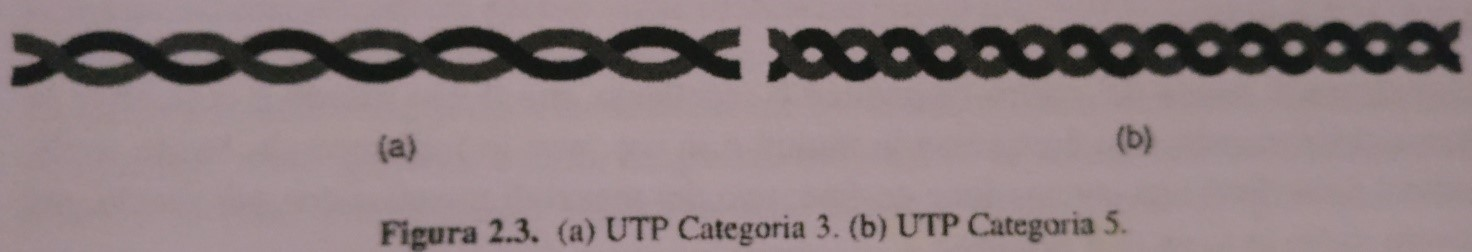
\includegraphics[scale=0.7]{res/img/3_Doppino.jpg}
%\caption{Didascalia dell'immagine}
\end{figure}

\textbf{Il cavo coassiale}: \\
-Cos’è: è un cavo composto da un nucleo conduttore coperto da un rivestimento isolante, a sua volta circondato da un conduttore cilindrico, solitamente realizzato con una calza di conduttori sottili, che infine è avvolto da una guaina protettiva di plastica. La costruzione e la schermatura del cavo coassiale forniscono ampiezza di banda ed eccellente immunità al rumore. Ne esistono di due tipi, a 50$\Omega$ per le trasmissioni digitali e a 75$\Omega$ per quelle analogiche; non c’è una motivazione tecnica per questa distinzione. \\
-Applicazione: Il cavo coassiale è molto utilizzato per le reti metropolitane e le televisioni via cavo; la banda disponibile dipende dalla qualità, dalla lunghezza del cavo e dal rapporto segnale-rumore del segnale dati. Per molti ambiti il cavo coassiale è stato sostituito dalla fibra ottica per i tratti più lunghi.

\begin{figure}[H]
\centering
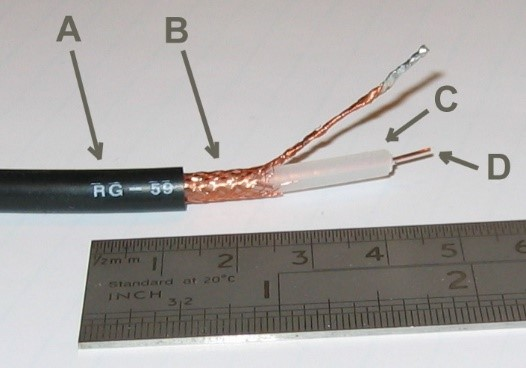
\includegraphics[scale=1]{res/img/3_cavoCoassiale.jpg}
\caption{D: nucleo, C: rivestimento isolante, B: conduttore cilindrico, A: guaina protettiva}
\end{figure}

\textbf{Fibra ottica:}\\
-Cos’è: Un sistema di trasmissione ottico è formato da: sorgente luminosa, mezzo di trasmissione e rilevatore. I cavi in fibra ottica sono il mezzo di trasmissione di questo sistema, che si basa su segnali luminosi invece che elettrici.
La fibra ottica è formata da un nucleo (core) di vetro, attraverso il quale si propaga la luce, ha uno spessore di 50 micron per le fibre multimodali mentre dagli 8 ai 10 micron per quelle monomodali.

Il nucleo è avvolto da un rivestimento di vetro (cladding) che ha un indice di rifrazione più basso; ciò costringe la luce a rimanere nel nucleo. L’ultimo strato è formato da plastica e serve a proteggere il rivestimento. Generalmente le fibre sono raggruppate in fasci, protetti da un’ulteriore guaina più esterna.  

\begin{figure}[H]
\centering
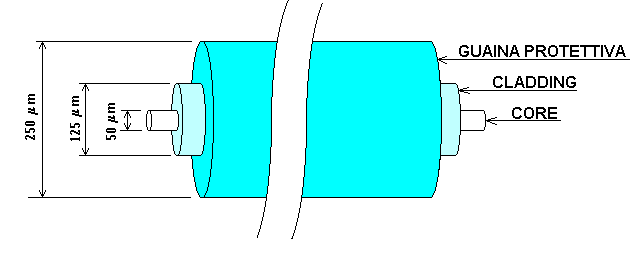
\includegraphics[scale=0.7]{res/img/3_FibraOttica.png}
%\caption{Didascalia dellimmagine}
\end{figure}

Esistono due tipi di fibra, la monomodale e la multimodale. La monomodale è più costosa e utilizzata soprattutto per le lunghe distanze, in cui la luce può propagarsi solo in linea retta senza rimbalzare.
Nella multimodale invece può contenere più raggi che rimbalzano ad angoli diversi, in questo caso si dice che ogni raggio ha una modalità diversa, da qui il nome multimodale.

Le fibre si possono collegare in diversi modi:
\begin{itemize}
\item Tramite connettori in apposite prese, perdono il 10-20\% di luce ma semplificano la riconfigurazione dei sistemi. 
\item Attaccate meccanicamente, tramite una manichetta speciale viene pinzato, viene poi allineato in modo da massimizzare il segnale, perdita del 10\% 
\item Fusione delle due parti, genera una piccola attenuazione.
\end{itemize}
-Applicazione: La fibra è molto utilizzata nelle LAN e nei sistemi di trasmissioni a lunga distanza e apporta diversi vantaggi rispetto al cavo in rame:
\begin{itemize}
\item	Maggiore ampiezza di banda.
\item	I ripetitori possono essere installati ogni 50km rispetto ai 5km dei cavi in rame, con un evidente risparmio.
\item	Non è influenzata da sorgenti elettriche, dai campi elettromagnetici e dalle interruzioni della linea elettrica, la fibra è adatta anche agli ambienti più inospitali.
\item	La fibra è sottile e leggera, occupando meno spazio permette alle aziende telefoniche di svuotare i condotti ormai saturi di cavi.
\item	Le fibre non perdono la luce ed è difficile intercettare i dati, questo le rendono molto più sicure rispetto ai cavi in rame.
\end{itemize}
Presenta tuttavia degli svantaggi, che nonostante tutto non limitano troppo questa tecnologia, che rappresenta il futuro per le telecomunicazioni. Tra gli svantaggi troviamo:
\begin{itemize}
\item	Tecnologia meno nota, richiede conoscenze che non tutti gli ingegneri possiedono.
\item	Si può danneggiare se la si piega troppo.
\item	La trasmissione è unidirezionale, di conseguenza, per avere una comunicazione bidirezionale è richiesta una doppia fibra o due bande di frequenza in una sola.
\item	Le interfacce per la fibra ottica costano di più di quelle elettriche.
\end{itemize}


\section{Caratteristiche e confronto tra i vari tipi di satellite: GEO, MEO e LEO}

Un satellite di comunicazioni può essere immaginato come un grande ripetitore di microonde posto nel cielo. Questo dispositivo contiene diversi transponder, ossia ricetrasmettitori satellitari, i quali ascoltano una parte dello spettro, amplificano il segnale e lo ritrasmettono su altre frequenze per evitare interferenze.

La collocazione dei satelliti è importante, e determinata da alcuni fattori:
\begin{itemize}
\item	Il periodo orbitale: più alto è il satellite, più lungo è il periodo.
\item	Le fasce di Van Allen distruggerebbero velocemente un satellite che le attraversasse.
\end{itemize}
Esistono quindi 3 zone in cui i satelliti possono essere collocati
\begin{itemize}
\item LEO: sotto la fascia di Van Allen inferiore
\item MEO: tra la fascia VA inferiore e quella superiore
\item GEO: molto al di sopra della fascia VA superiore
\end{itemize}

\begin{figure}[H]
\centering
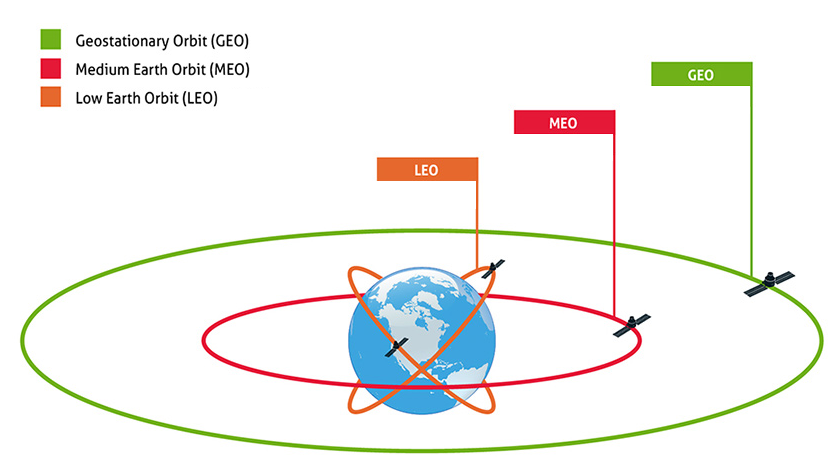
\includegraphics[scale=0.55]{res/img/4_satelliti.png}
\end{figure}
 
\paragraph{GEO}
GEO (Geostationary Earth Orbit), sono collocati nella fascia più alta, disposti con un intervallo di $2^{\circ}$ nel piano equatoriale, così da evitare interferenze, di conseguenza c’è posto per “solo” 180 satelliti di questo tipo, la loro dimensione è importante e la gestione dell’allocazione degli slot orbitali è motivo di disputa tra paesi, stazioni televisive e militari.
\paragraph{MEO}
Tra le due fasce di Van Allen troviamo i satelliti MEO (Medium Earth Orbit), questi satelliti si spostano lentamente lungo la longitudine, impiegando 6 ore per compiere un giro attorno al pianeta, attualmente non sono utilizzati per le telecomunicazioni. Rispetto al GEO, il MEO permette un ritardo di propagazione inferiore, tuttavia si perde la comodità del “punto fisso” garantito dal GEO, questo perché il MEO si sposta più velocemente.
\paragraph{LEO}
I LEO (Low Earth Orbit) sono i più bassi tra i tre tipi; si spostano molto velocemente, di conseguenza un sistema completo richiede l’utilizzo di molti satelliti di questo tipo. D’altra parte, le stazioni terrestri non hanno bisogno di molta energia per la comunicazione e i ritardi sono di pochi millisecondi.
Questo tipo di satellite tratta prevalentemente trasmissione voce e servizi internet/GPS. \\

Una menzione particolare va fatta alla differenza tra satelliti e fibra: quale preferire? \\
Non esiste una risposta ben definita, la fibra grazie alla sua comodità sembrava avesse preso dominio nel mercato, tuttavia i satelliti avevano applicazione in campo in cui la fibra non poteva arrivare:
\begin{itemize}
\item	La fibra non è attualmente disponibile a una gran parte dell’utenza, mentre per i satelliti, l’utente basta che innalzi un’antenna sul tetto di casa per ottenere una maggiore ampiezza di banda.
\item	Comunicazione mobile, la fibra ottica non è di nessuna utilità per questa categoria, mentre i collegamenti satellitari potenzialmente ce l’hanno.
\item	Comunicazione broadcast, un messaggio inviato da un satellite può essere ricevuto contemporaneamente da migliaia di stazioni terrestri.
\item	Comunicazione in luoghi con terreni inospitali o scarsamente dotati di infrastrutture.
\end{itemize}
Il sistema di comunicazione principale del futuro sarà quello terrestre basato su fibre ottiche, combinato con la rete radio cellulare, tuttavia per alcune applicazioni specifiche i satelliti sono migliori.


\section{Cos’è la modulazione in frequenza?}
Durante l’invio di informazioni, il segnale può subire attenuazione, distorsione o venir disturbata dal rumore; questo porta ad evitare l’uso di un largo intervallo di frequenze, ma sfortunatamente le onde quadre utilizzate nei segnali digitali utilizzano un ampio spettro di frequenza, e perciò sono soggette ad una forte attenuazione e alla distorsione.

Questi effetti rendono adatta la trasmissione in banda base (DC) solo a velocità basse e distanze brevi.

Per aggirare questi problemi viene usata la trasmissione AC, un tono continuo (portante d’onda sinusoidale) nell’intervallo compreso tra 1000 e 2000Hz, il quale permette la modulazione della sua ampiezza (AM), frequenza (FM) o fase.

\begin{figure}[H]
\centering
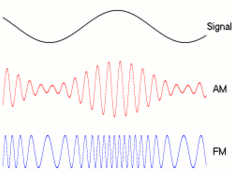
\includegraphics[scale=1]{res/img/5_modulazione.png}
\end{figure}

La modulazione in frequenza non è altro che una tecnica di trasmissione utilizzata per trasmettere informazioni usando la variazione di frequenza dell’onda portante. Rispetto alla modulazione in ampiezza ha il vantaggio di essere molto meno sensibile ai disturbi e permette una trasmissione di miglior qualità. Ha inoltre un’efficienza energetica molto maggiore dato che la potenza del segnale modulato FM è esclusivamente quello della portante.

Il difetto principale è la necessità di circuiti più complessi, sia per la generazione del segnale sia per la ricezione. L’attuale tecnologia ha permesso di superare queste problematiche, rendendo la modulazione in frequenza molto più usata rispetto a quella in ampiezza, soprattutto in ambito di broadcasting commerciale.

\section{Cos’è la modulazione delta (delta modulation)?}
La delta modulation è un metodo di digitalizzazione e compressione di un segnale analogico.
Si basa sul fatto che il segnale cambia in modo relativamente lento rispetto alla frequenza di campionamento, ciò rende gran parte dell’informazione ridondante.

Questo metodo prevede che ogni valore campionato differisca dal precedente di +1 o -1, sotto queste condizioni è possibile trasmettere un singolo bit che dice se il nuovo campione è maggiore o minore del precedente.

Un problema si ha se il segnale cambia troppo rapidamente, in quel caso si perdono informazioni.

\begin{figure}[H]
\centering
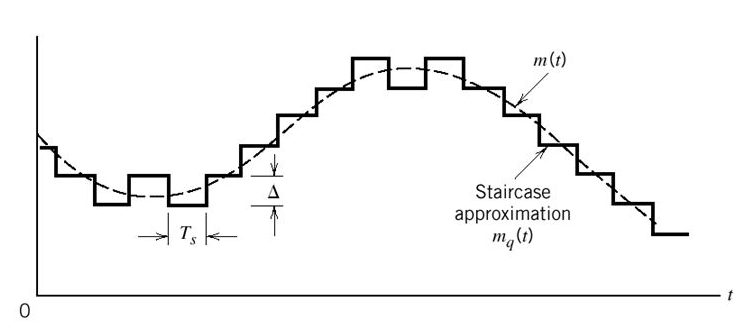
\includegraphics[scale=0.6]{res/img/6_modulazioneDelta.png}
\end{figure}
 
\section{Descrivere in dettaglio il GSM (Global System for Mobile connection)}
Esistono tre generazioni distinte di telefoni cellulari ognuna caratterizzata da una diversa tecnologia:
\begin{itemize}
\item	Voce analogica
\item	Voce digitale
\item	Voce e dati digitali (Internet, posta elettronica ecc.)
\end{itemize}
Il GSM tratta dei telefoni della seconda generazione: voce digitale.
La sua struttura è formata da 4 tipi di celle: macro, micro, pico e umbrella. 
Le prime sono le più grandi, sono sopraelevate rispetto gli edifici e hanno un raggio massimo di 35 km. Le micro sono più piccole, coprono un'altezza pari agli edifici. Le pico sono molto piccole, usate in aree molto dense, tipicamente indoor. Umbrella è una piccola estensione, usata per coprire i buchi tra le varie celle sopracitate.

Sfrutta il multiplexing a divisione di frequenza, con ogni apparecchio che trasmette su una frequenza e riceve su una frequenza più alta. Una singola coppia di frequenza è divisa in slot temporali e condivisa tra più utenti attraverso un meccanismo di multiplexing a divisione di tempo.

Questi fattori lo rendono molto simile al D-AMPS, tecnologia molto utilizzata in America, che condivide la stessa generazione di telefoni. Tuttavia, GSM sono molto più ampi di quelli AMPS e contengo un numero poco più alto di utenti, perciò la velocità dati per utente di GSM è superiore a quella di D-AMPS.

Un sistema GSM ha 124 coppie di canali simplex e supporta otto connessioni separate mediante multiplexing a divisione di tempo.
A ogni stazione attiva è assegnato uno slot temporale su una coppia di canali.

Trasmissione e ricezione non avvengono nello stesso intervallo temporale perché GSM non è in grado di trasmettere e ricevere contemporaneamente.

Il GSM introduce anche l’utilizzo della SIM card, in cui vengono memorizzati i dati descrittivi dell’abbonato e ha la funzione principale di fornire autenticazione ed autorizzazione all’utilizzo della rete.

\section{Si descriva la tecnica CDMA (Code Division Multiple Access), possibilmente con esempio}
Esistono tre generazioni distinte di telefoni cellulari ognuna caratterizzata da una diversa tecnologia:
\begin{itemize}
\item	Voce analogica
\item	Voce digitale
\item	Voce e dati digitali (Internet, posta elettronica ecc.)
\end{itemize}
Il CDMA tratta dei telefoni della seconda generazione: voce digitale.
D-AMPS e GSM sono sistemi che utilizzano FDM e TDM per dividere lo spettro in canali e i canali in slot temporali. CDMA invece di dividere l’intero intervallo di frequenze assegnate in poche centinaia di canali a banda stretta, permette ad ogni stazione di trasmettere per tutto il tempo attraverso l’intero spettro di frequenza. Trasmissioni multiple simultanee sono separate usando la teoria della codifica. La capacità del CDMA è di riuscire a estrarre il segnale desiderato scartando tutto il resto.

In CDMA, ogni tempo bit è suddiviso in m intervalli chiamati chip. In genere ci sono 64 o 128 chip per ogni bit. Ad ogni stazione è assegnato un codice di m-bit univoco chiamato sequenza di chip.
Per trasmettere un bit 1, una stazione invia la sua sequenza di chip; per trasmettere un bit 0 la stazione invia il complemento a uno della propria sequenza di chip.
Ogni stazione adotta una sequenza di chip univoca.

CDMA rispetto a GSM e D-AMPS opera in una banda di 1,25MHz, permettendo agli utenti di avere un’ampiezza di banda considerevole.
Una sequenza di chip e il suo contrario sono a due a due ortogonali (il prodotto interno normalizzato è 0). Per generare queste sequenze di frammento ortogonali si utilizza un metodo noto come codici Walsh. 
Se la sequenza di chip ricevuta è S e il ricevitore sta cercando di ascoltare una stazione la cui sequenza di chip è C, il prodotto interno normalizzato da calcolare è S*C; facendo i calcoli si possono eliminare i termini superflui grazie all’ortogonalità dei valori, estraendo correttamente il valore trasmesso da C. 
Ad esempio, A e C trasmettono 1, B trasmette 0. Il ricevitore vede la somma S=A+!B+C e calcola:
\begin{center}
$S*C=(A+!B+C)*C=A*C+B*C+C*C=0+0+1=1$
\end{center}
I primi due termini spariscono perché le sequenze di chip sono state scelte per essere ortogonali.

\section{Il GPRS: Cos’è? Pregi e difetti}

Esistono tre generazioni distinte di telefoni cellulari ognuna caratterizzata da una diversa tecnologia:
\begin{itemize}
\item	Voce analogica
\item	Voce digitale
\item	Voce e dati digitali (Internet, posta elettronica ecc.)
\end{itemize}
GPRS è un’evoluzione tra la seconda e la terza generazione di telefoni cellulari. È una rete a pacchetti costruita sopra D-AMPS e GSM. Questa permette alle stazioni mobili di inviare e ricevere pacchetti IP in una cella basata su un sistema vocale.

Quando GPRS è operativo vengono riservate alcuni slot temporali posti su alcune frequenze, per il traffico di pacchetti.
Gli slot disponibili sono divisi in canali logici, la stazione base determina l’associazione tra i canali logici e time slot. Un canale logico è usato per scaricare i pacchetti dalla stazione base nella stazione mobile e ogni pacchetto indica il destinatario.

Per inviare un pacchetto IP, una stazione mobile chiede uno o più slot inviando una richiesta alla stazione base. Se la richiesta arriva senza problemi, la stazione comunica all’apparecchio mobile la frequenza e gli slot che dovrà utilizzare per trasmettere il pacchetto. Una volta arrivato alla stazione base, il pacchetto è trasferito su Internet attraverso una connessione via cavo.

I vantaggi rispetto ai suoi predecessori stanno nel fatto che lo spreco di banda inesistente e viene utilizzata una tariffa a traffico e non a tempo. GPRS aggiunge il supporto a PPP e IP.

\section{Handoff cos’è e vari tipi}

Nell’ambito della telefonia mobile, con “Handoff” si intende la procedura per la quale un terminale cambia il canale (frequenza e slot di tempo) che sta utilizzando durante una comunicazione.

Un’area geografica è divisa in celle, al centro di ogni cella si trova una stazione base che comunica con tutti i telefoni che si trovano nella cella.

Quando un telefono mobile abbandona fisicamente una cella perché si accorge che il segnale si sta affievolendo, la stazione base di quella cella verifica il livello di potenza del segnale ricevuto dalle stazioni nelle celle adiacenti. A questo punto la stazione trasferisce la gestione dell’apparecchio alla cella che riceve il segnale più forte, ossia alla cella in cui ora si trova il telefono.
Il telefono viene informato della nuova centrale di controllo e viene forzato al cambiamento, questo è l’handoff.

Esistono due tipi di handoff: il soft e l’hard handoff. Nel soft handoff il telefono è acquisito dalla nuova stazione di base prima di interrompere il segnale precedente, il vantaggio sta nel fatto che non vi è nessuna perdita di continuità, tuttavia il telefono deve riuscire a gestire più frequenze nello stesso momento (né i telefoni di prima generazione ne seconda sono in grado).

Nel caso di hard handoff la vecchia stazione di base rilascia il telefono prima che la nuova lo acquisisca. Se la nuova non è in grado di prendere il controllo del dispositivo (ad esempio se non è disponibile nessuna frequenza) il segnale viene interrotto bruscamente, con il risultato di terminazione brusca di una possibile chiamata.



\section{FDM, TDM, CDM: Algoritmi per la selezione della banda}

\paragraph{FDM (Frequency Division Multiplexing)} è una tecnica di condivisione delle risorse trasmissive di un canale di comunicazione. L’intero canale trasmissivo disponibile è diviso in sotto canali, ognuno costituito da una banda di frequenza e separato da un altro grazie ad un piccolo intervallo di guardia.
Questo permette la condivisione dello stesso canale da parte di dispositivi che utilizzano diverse regioni di frequenze e utenti che possono cosi comunicare contemporaneamente senza interferirsi tra loro.
Questa tecnica è comunemente utilizzata nelle trasmissioni televisive, radiofoniche, telefoniche o di dati. Anche le reti cellulari utilizzano in parte questo tipo di multiplazione per suddividere e assegnare l’intera capacità trasmissiva o banda radio disponibile alle varie celle di copertura servite da stazion0.8i radio base.

\begin{figure}[H]
\centering
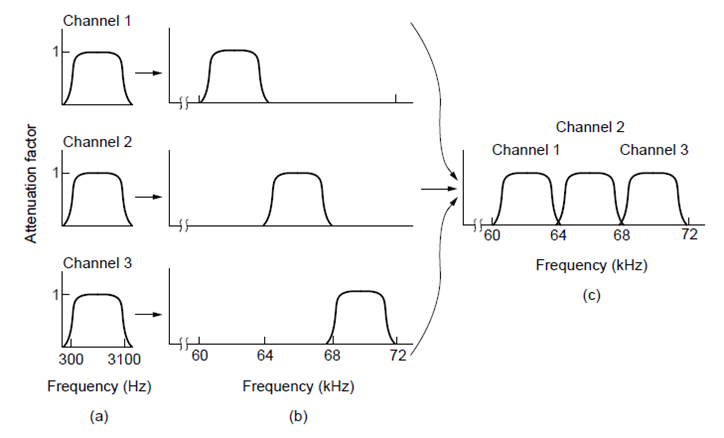
\includegraphics[scale=0.45]{res/img/11_FDM.png}
%\caption{Didascalia dellimmagine}
\end{figure}
 
\paragraph{TDM (Time Division Multiplexing)} è una tecnica di condivisione di un canale di comunicazione secondo la quale ogni dispositivo ricetrasmittente ottiene a turno l’uso esclusivo dello stesso per un breve lasso di tempo. Il tempo di utilizzo del canale è diviso in frame tutti della stessa durata, questi frame sono ulteriormente divisi in slot.
Confrontato all’FDM il TDM risulta essere più efficiente in quanto elimina la necessità degli intervalli di guardia o separazione tra le varie bande di frequenza. Necessita tuttavia di un circuito di sincronizzazione temporale in ricezione per l’estrazione del time-slot di competenza.

\begin{figure}[H]
\centering
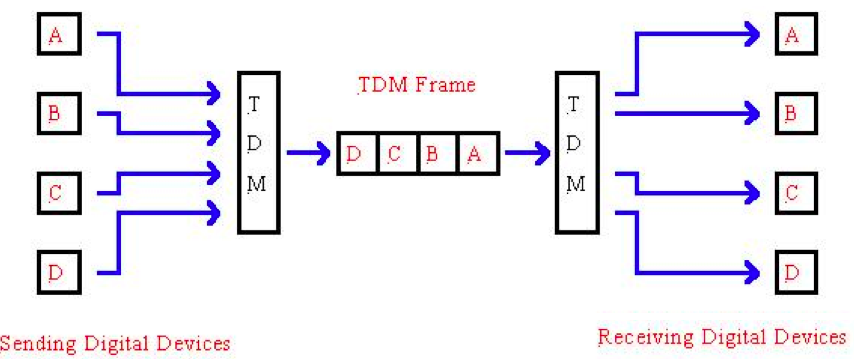
\includegraphics[scale=0.5]{res/img/11_TDM.png}
%\caption{Didascalia dellimmagine}
\end{figure} 

\paragraph{CDM (Code Division Multiplexing)} o conosciuta anche come CDMA è il protocollo di accesso multiplo a canale condiviso. Offre una maggiore velocità di trasmissione di dati rispetto a TDM e FDM.
Questa tecnica è realizzata moltiplicando in trasmissione l’informazione generata per un’opportuna parola detta chip; la sequenza in uscita dal moltiplicatore sarà successivamente modulata e infine trasmessa sul canale.
In ricezione il segnale ricevuto sarà costituito dalla somma vettoriale di tutti i segnali trasmessi dalle singole stazioni. Grazie all’ortogonalità dei chip delle sorgenti, l’estrazione dell’informazione associata a ciascuna sorgente potrà essere fatta moltiplicando il segnale ricevuto con il particolare codice associato alla determinata sorgente che si vuole estrarre.
La miglior efficienza rispetto alle precedenti forme di multiplazione è dovuta al fatto che ciascun canale utilizza l’intera banda di frequenza assegnata al servizio per tutto il tempo che desidera, e la non-interferenza è assicurata grazie all’uso di codici ortogonali.

\begin{figure}[H]
\centering
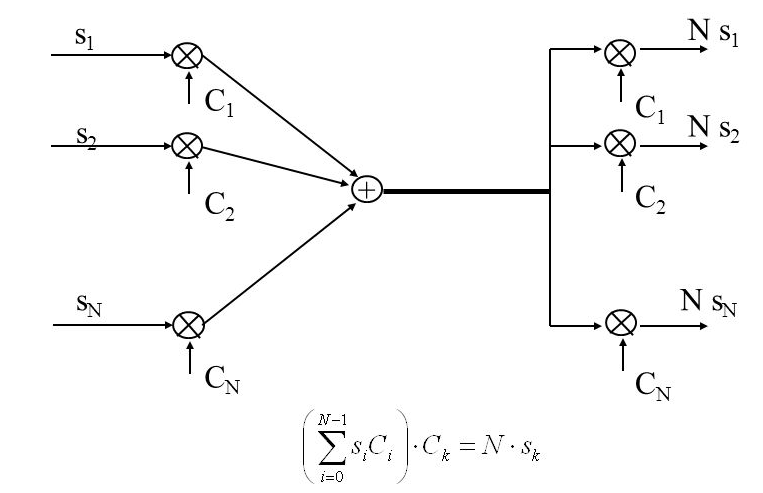
\includegraphics[scale=0.5]{res/img/11_CDM.png}
%\caption{Didascalia dellimmagine}
\end{figure}
 
\section{QAM e QAM16}

QAM è un sistema di modulazione numerica di ampiezza in quadratura, sia digitale che analogica. 
Le portanti sono sinusoidi. Il termine quadratura indica che differiscono di $90^{\circ}$.
Il segnale in ingresso viene suddiviso e modulato per l’ampiezza. Nel caso di segnali digitali si sommano i segnali modulati e si ottiene una forma d’onda che risulta una combinazione della modulazione di fase e quella d’ampiezza.
Ciascun tipo di modulazione QAM è caratterizzato da un diagramma (costellazione) su cui sono rappresentati tutti gli stati della portante.
La QAM, rispetto alla PSK (Phase shift keying), migliora l’immunità al rumore.
QAM16 non è altro che un tipo di costellazione del QAM, utilizzando quattro ampiezze e quattro fasi, per un totale di 16 diverse combinazioni. Ogni modem ad alta velocità ha un suo schema di costellazione e può comunicare solo con altri modem che adottano lo stesso schema (anche se generalmente un modem riesce a emulare anche quelli più lenti).

\begin{figure}[H]
\centering
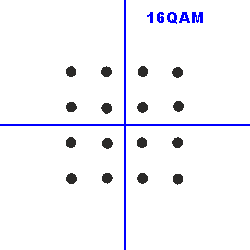
\includegraphics[scale=0.6]{res/img/12_QAM16.png}
%\caption{Didascalia dellimmagine}
\end{figure}
 
\section{Cos’è il byte stuffing?}

Lo strato data link deve servire lo stato network, per farlo necessita di usare a sua volta le informazioni fornite dallo strato fisico il cui scopo è quello di prendere un flusso di bit e cercare di portarli a destinazione.
Non esiste nessuna garanzia per la correttezza dei dati, i bit potrebbero essere maggiori, minori, modificati ecc. Uno dei compiti dello strato data link è quello di rilevare ed eventualmente correggere questi errori.
Il modo per rinvenire questi errori è quello di suddividere il flusso dei bit in frame, per poi controllarli, uno dei metodi di framing è quello di utilizzare un flag byte con il byte stuffing.
Il byte stuffing prevede l’uso di un flag per delimitare l’inizio e la fine dei frame. In questo modo quando il destinatario perde la sincronizzazione può cercare il flag byte per trovare la fine del frame corrente. Due flag byte consecutivi indicano la fine di un frame e l’inizio del successivo.
Per far si che un flag byte sia contenuto internamente ai dati, bisogna utilizzare un byte di escape (ESC) prima di ogni occorrenza “accidentale” del byte flag nei dati. Successivamente lo strato data link della destinazione provvederà a rimuovere i byte di escape prima di passare i dati allo strato network, se anche un carattere ESC si trova dentro i dati, va preceduto da un ulteriore carattere ESC.
Questo metodo di framing presenta notevoli svantaggi, in primis quello di essere legato all’uso di caratteri da 8 bit, non tutte le codifiche dei caratteri li usano. Un altro problema deriva dalla quantità di caratteri superflui da inserire per effettuare lo stuffing, per questo si è sentita la necessità di sviluppare una nuova tecnica di framing che consente di gestire caratteri di lunghezza arbitraria (bit stuffing).
Il byte stuffing è usato in PPP (Point-to-Point Protocol).

\begin{figure}[H]
\centering
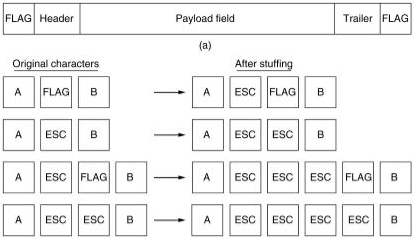
\includegraphics[scale=0.8]{res/img/13_ByteStuffing.png}
%\caption{Didascalia dellimmagine}
\end{figure}

\section{Cos’è il bit stuffing?}

Lo strato data link deve servire lo stato network, per farlo necessita di usare a sua volta le informazioni fornite dallo strato fisico il cui scopo è quello di prendere un flusso di bit e cercare di portarli a destinazione.
Non esiste nessuna garanzia per la correttezza dei dati, i bit potrebbero essere maggiori, minori, modificati ecc. Uno dei compiti dello strato data link è quello di rilevare ed eventualmente correggere questi errori.
Per risolvere i problemi e le limitazioni provocate dal byte stuffing, viene sviluppata una nuova tecnica di framing , che prende il nome di bit stuffing, questa nuova tecnica permette di creare data frame che contengono sia un numero arbitrario di frame, sia codifiche di carattere con un numero arbitrario di bit.
Ogni frame comincia e finisce con un gruppo speciale di bit “0111110” (flag byte). Ogni volta che lo strato data link della sorgente incontra cinque “1” consecutivi nei dati inserisce automaticamente un bit con valore 0 nel flusso in uscita. La destinazione quindi quando riceve cinque bit consecutivi con valore 1 seguiti da uno 0, automaticamente elimina lo 0.
Con il bit stuffing il confine fra i due frame viene riconosciuto in modo inequivocabile tramite l’uso della sequenza flag.
 
\begin{figure}[H]
\centering
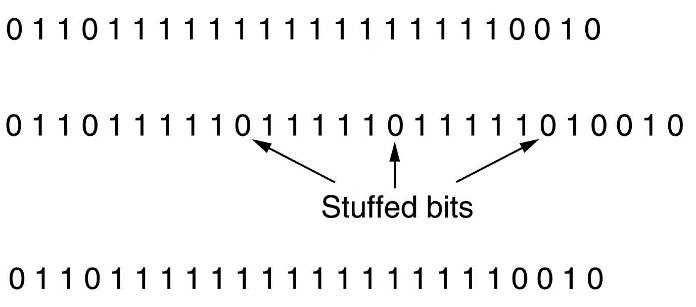
\includegraphics[scale=0.8]{res/img/14_BitStuffing.png}
%\caption{Didascalia dellimmagine}
\end{figure}

\section{Numero di bit necessari per riconoscimento (correzione) degli errori di trasmissione?}

I dati trasmessi nei collegamenti locali sono spesso soggetti ad errori, per la loro gestione sono state sviluppate due strategie di base: la prima si basa su una codifica a correzione d’errore mentre la seconda è una codifica a rilevazione d’errore.
La prima introduce una ridondanza (in ciascun blocco trasmesso) tale da riuscire a ricostruire il messaggio in caso di anomalie. La seconda invece introduce ridondanza sufficiente solo a capire che c’è stato un errore, ma non di correggerlo.
Un frame generalmente consiste di m bit di dati e r bit ridondanti per i controlli, la somma n=m+r è la lunghezza totale del frame chiamata codeword di n bit. Date due codeword, per capire quanti bit corrispondenti sono differenti bisogna effettuare l’OR esclusivo e contare il numero di bit a “1” nel risultato, questo numero è chiamato distanza di Hamming.
Detto questo, per trovare d errori è necessaria una codifica con distanza d+1, quando la destinazione vede una codeword non valida riesce a determinare che c’è stato un errore, ma non a correggerlo.
Per correggere d errori è necessaria una codifica con distanza 2d+1, in tal modo codeword legali sono distanziate in modo tale che anche con d cambiamenti la codeword originale è sempre più vicina di ogni altra, può quindi essere determinata univocamente.
Un semplice esempio di codifica a rilevazione d’errore si può realizzare aggiungendo un bit di parità ai dati, calcolato in modo che il numero di “1” nella codeword sia sempre pari (o dispari).
Entrambe le codifiche trovano uso in diversi ambienti:
Nelle reti wireless, in cui è presente molto rumore, conviene utilizzare una codifica a correzione d’errore, cosi da ricostruire il messaggio in caso di errori, invece di farselo rispedire rischiandone di ulteriori. 
Sui canali affidabili invece è più economico usare codifiche a rilevazione, ed eventualmente farsi ritrasmettere il blocco.
Questo perché, anche come visto dalla formula, per correggere gli errori abbiamo bisogno di molti più bit rispetto ad accorgersene solamente.

\section{Si descriva cos'è il CRC (Cycle Redundancy check). Si calcoli inoltre il CRC di 10011101 usando il polinomio generatore di $x^4+x+1$}

Il CRC o Cycle Redundancy Check, è un metodo per il calcolo di somme di controllo, serve a individuare errori casuali nella trasmissione di dati (causati da interferenze, rumori di linea o distorsione). Non è utile invece nel caso di tentativi intenzionali di manomissione.
Il CRC tratta le sequenze di bit come dei polinomi a coefficienti che possono assumere solo valori “0” o “1”. Un frame di k bit è visto come una lista di coefficienti per un polinomio con k termini che variano da $x^k-1$ a $x^0$. Questo polinomio è detto di grado k-1 e il coefficiente più alto è quello più a sinistra del polinomio (es 110001 ha 6 bit, quindi rappresenta un polinomio di $5^{\circ}$ grado con coefficienti 1,1,0,0,0 e 1: $x^5+x^4+x^0$.

Quando si utilizza una codifica di questo tipo, sorgente e destinazione devono mettersi d’accordo in anticipo su un polinomio generatore G(x). Che deve avere i bit di ordine più alto e più basso a “1”.
Per poter calcolare il checksum di un frame di m bit, quest’ultimo dev’essere più lungo del polinomio generatore. L’idea è quella di aggiungere un checksum alla fine del frame in modo che il polinomio rappresentato dal frame con checksum sia divisibile per G(x). Quando la destinazione riceve il frame con il checksum e prova a dividerlo per G(x). Se c’è un resto vuol dire che c’è stato un errore di trasmissione.
Ora proviamo con l’esempio di un frame 10011101 con polinomio generatore $x^4+x+1$:
Frame: 1 0 0 1 1 1 0 1 
Generatore G(x): 1 0 0 1 1
Il grado di G(x) è 4, aggiungo 4 “0” al frame (ottenendo un nuovo frame M(x)) in modo da poter dividere le due parti ottenendo il resto da sottrarre al M(x).
M(x)= 1 0 0 1 1 1 0 1 0 0 0 0
Effettuo la divisione: 

\begin{figure}[H]
\centering
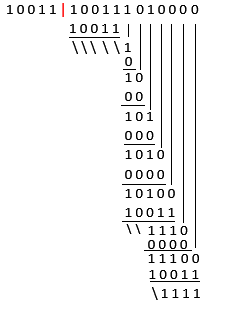
\includegraphics[scale=0.65]{res/img/16_DivisioneEsCRC.png}
%\caption{Didascalia dellimmagine}
\end{figure}
             
1 1 1 1 è il resto di conseguenza, il frame trasmesso è 1 0 0 1  1 1 0 1  1 1 1 1.

\section{Descrivere il protocollo stop-and-wait, pregi e difetti}

Durante la ricezione dei dati, il frame viene controllato, e a seconda se è integro o meno, si segue uno dei tre diversi protocolli più comuni: 
Stop-and-wait è il più semplice tra questi.
Un mittente manda solo un frame alla volta, il destinatario, dopo aver ricevuto il frame corretto, invia un ACK (Acknowledge) al mittente, che a sua volta provvede a spedire il secondo frame e cosi via. 
Se l’ACK non raggiunge il mittente, questo provvederà a inviare nuovamente lo stesso frame dopo aver atteso un certo tempo (timeout).
Altri problemi sorgono quando l’ACK arriva danneggiato, in quel caso il mittente invia nuovamente il frame, con il risultato che il destinatario si trova due frame uguali, senza sapere se è un duplicato o se effettivamente il pacchetto successivo ha gli stessi dati, per questo è stato implementato un numero di sequenza per i frame, e il destinatario invia l’ACK inerente a quel frame.
Anche in questo caso sorgono problemi di dissincronia, in cui, sbagliando i numeri dei frame si rischia di perderne molteplici.
Concludendo lo stop-and-wait è parecchio inefficiente rispetto agli altri protocolli di “comunicazione di richiesta di ripetizione automatica”, specialmente a causa del tempo che intercorre tra l’invio dei vari pacchetti e contando anche il fatto che essendoci gli ACK il tempo di comunicazione aumenta considerevolmente, limitando la capacità del canale di comunicazione.
 
\begin{figure}[H]
\centering
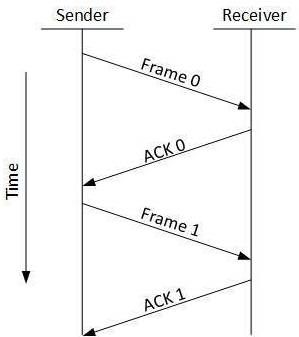
\includegraphics[scale=0.65]{res/img/17_StopAndWait.png}
%\caption{Didascalia dellimmagine}
\end{figure}
	     
\section{Cos’è il piggybacking?}

Molti protocolli di comunicazione necessitano di inviare l’ACK come segnale di avvenuta ricezione del frame.
Fatto per ogni singolo frame, questo invio rischia di intasare inutilmente il canale di comunicazione, allungando i tempi e incorrendo in molteplici errori.
La tecnica del piggybacking permette di aggiungere l’ACK al frame di dati in uscita, utilizzando il campo ack nell’intestazione di questo. In questo modo l’acknowledgement si procura un passaggio gratis insieme al successivo frame dati trasmesso.
Questo avviene quando arriva un frame di dati, la destinazione non invia subito un frame di controllo separato, ma aspetta che lo strato network gli passi il successivo pacchetto.
Un problema può sorgere in caso di attesa molto lunga del pacchetto, poiché si rischia di far scattare il timer del mittente che re-invia il frame nell’attesa dell’ACK, in questo caso si decide un timeout in modo tale da fare piggybacking nel caso in cui il pacchetto da inviare è pronto in tempi celeri, altrimenti si invia l’ACK in modo indipendente.
Il vantaggio principale sta nel miglior uso della banda disponibile, inoltre un minor numero di frame inviati significa anche un minor numero di interrupt “frame in arrivo”, con conseguente minor necessità di buffer.

\section{Si descriva la tecnica dello Sliding window}

Sliding window è una classe di protocolli di controllo di flusso di dati, usato in particolare dal TCP.
Una sliding window è formata da una finestra di invio e da una finestra di ricezione. La prima indica i frame che è autorizzata ad inviare, la seconda invece corrisponde all’insieme dei frame che può accettare.
La finestra di invio contiene i frame da spedire, o spediti ma in attesa di ack, lo scopo è quello di mantenere nel buffer più frame, in modo da ritrasmetterli in caso di problemi. Se questo buffer è pieno, il livello data link costringe il livello network a sospendere la consegna di pacchetti. Quando si ottiene un ack il frame corrispondente esce dalla finestra lasciando posto ad altri.
Analogamente, il destinatario mantiene una finestra corrispondente agli indici dei frame che possono essere accettati, se arriva un frame il cui indice è fuori dalla finestra questo viene scartato (senza invio dell’ack). Se l’indice è dentro la finestra, il frame viene accettato, viene spedito l’ack e si sposta in avanti la finestra.
Le finestre di mittente e destinatario non devono avere necessariamente uguali dimensioni.

\begin{figure}[H]
\centering
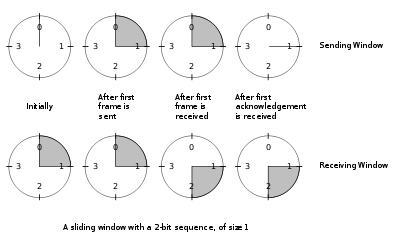
\includegraphics[scale=1]{res/img/19_SlidingWindow.png}
%\caption{Didascalia dellimmagine}
\end{figure}
 
Si noti che nel caso in cui abbiamo una finestra di dimensione massima uguale a 1 ci troviamo nel caso stop-and-wait, ovvero, dopo aver inviato un frame si attende l’ack corrispondente prima di inviarne ulteriori. In questo caso si mantiene l’ordine, con finestre più larghe questo non è più vero.

\section{Si descriva l'idea dei protocolli "go back N", indicandone pregi e difetti}

Il problema di ricezione dell’ack per ogni frame inviato, limitava di molto l’utilizzo della banda e rallentava le comunicazioni, per ovviare a questo problema viene usata la tecnica di pipelining. Si decide quindi di inviare più frame prima di ricevere i vari ack aumentando di parecchio l’utilizzo della linea. Tuttavia, sorge un problema, cosa succede nel caso in cui si perdano dei frames? Per il ripristino degli errori in presenza di pipelining sono disponibili due approcci base.

Tra questi go back n. Go back n è un’istanza specifica del protocollo “Automatic Repeat-reQuest” (modalità di trasmissione di pacchetti di dati) nel quale il processo mittente continua a mandare un numero di frame specificato nella window size anche senza aver ricevuto nessun ACK.
La strategia corrisponde ad una finestra in ricezione di dimensione 1, rilevato l’errore si rifiuta di accettare qualunque frame eccetto il successivo che deve inviare allo strato network. Per questo il mittente scaduto il timeout riprende a spedire i frames che non hanno ricevuto l’ack.
Questa tecnica può essere ottimizzata dall’uso del piggybacking, che consiste nello scrivere l’ack di un pacchetto nell’intestazione del pacchetto di informazione successivo, evitando latenze di trasmissione dovute alla trasmissione del solo ack.
Go back n è uno dei metodi più efficienti per effettuare una connessione in quanto spedisce più pacchetti senza attendere ack, migliorando l’uso della banda, tuttavia può far perdere molta banda se la frequenza degli errori è molto alta.
Go back-n e il selective repeat hanno diverse conseguenze in termini di uso di banda e di spazio di buffer nello strato data link, si può utilizzare un approccio oppure un altro in base a quale risorsa è più scarsa.

\begin{figure}[H]
\centering
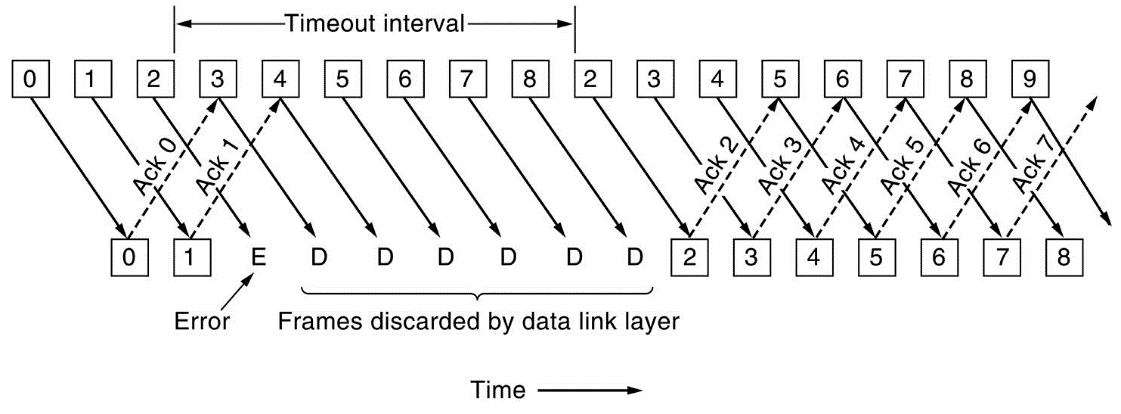
\includegraphics[scale=0.9]{res/img/20_GoBackN.png}
%\caption{Didascalia dellimmagine}
\end{figure} 

\section{Si descriva cos'è la tecnica del selective repeat}

Il problema di ricezione dell’ack per ogni frame inviato, limitava di molto l’utilizzo della banda e rallentava le comunicazioni, per ovviare a questo problema viene usata la tecnica di pipelining. Si decide quindi di inviare più frame prima di ricevere i vari ack aumentando di parecchio l’utilizzo della linea. Tuttavia, sorge un problema, cosa succede nel caso in cui si perdano dei frames? Per il ripristino degli errori in presenza di pipelining sono disponibili due approcci base.

Tra questi troviamo il selective repeat, usando questo metodo quando viene ricevuto un frame in errore viene scartato, mentre i frame buoni ricevuti successivamente vengono salvati in un buffer, quando la sorgente va in timeout, solo il frame più vecchio senza ack viene ritrasmesso. Se quel frame arriva correttamente, la destinazione può passare in sequenza allo strato network tutti i frame presenti nel buffer.
La ripetizione selettiva può inviare dei NACK (Not acknowledgement) quando trova un errore, cosi da stimolare la ritrasmissione prima dello scadere del timer.
La ripetizione selettiva corrisponde ad avere una finestra di ricezione maggiore di 1.
Go back-n e il selective repeat hanno diverse conseguenze in termini di uso di banda e di spazio di buffer nello strato data link, si può utilizzare un approccio oppure un altro in base a quale risorsa è più scarsa.

\begin{figure}[H]
\centering
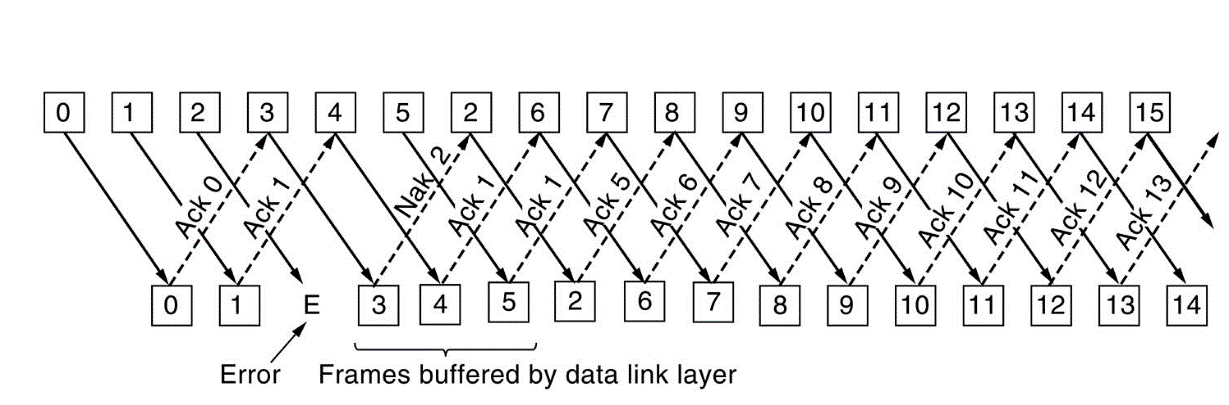
\includegraphics[scale=0.8]{res/img/21_SelectiveRepeat.png}
%\caption{Didascalia dellimmagine}
\end{figure}
 
\section{Descrivere la differenza tra ALOHA e ALOHA-SLOTTED}

ALOHA è un protocollo di rette per garantire le funzionalità di accesso multiplo al mezzo di trasmissione dati condiviso tra più utenti. Esistono due tipi di reti: quelle che utilizzano le connessioni punto-punto e quelle che usa canali broadcast, questo protocollo viene utilizzato per le seconde.
Inventato negli anni ’70 nelle Hawaii, l’idea di fondo è di consentire agli utenti di trasmettere ogni volta che hanno dati da inviare. Questo naturalmente genera collisioni, tuttavia poiché i canali broadcast danno la possibilità di verificare se il frame trasmesso è stato ricevuto correttamente o no, la stazione trasmittente ascolta il canale e determina il successo o insuccesso della trasmissione.
Le stazioni attendono un tempo variabile prima di provare a ritrasmettere un frame non andato a buon fine.
Il successo dell’ALOHA puro è di circa 18\%.
Il protocollo Slotted ALOHA aggiunge al protocollo sopracitato la divisione del tempo in intervalli discreti, chiamati slot. Ogni stazione viene vincolata a cominciare la propria trasmissione solo all’inizio di uno slot temporale, se una stazione è pronta ad un certo istante, dovrà necessariamente attendere l’inizio dello slot successivo.
Lo svantaggio di questo protocollo è la necessità di un meccanismo di sincronizzazione che indichi alle varie stazioni quando possono cominciare la trasmissione.
Questa divisione in slot migliora il grado di successo del doppio rispetto all’ALOHA puro, circa 36\%.
Questi risultati non dovrebbero sorprendere, in quanto con stazioni che trasmettono a piacimento è molto facile incorrere in collisioni.
Subito dopo l’invenzione, questi protocolli caddero in disuso, fino a quando non si presentò il problema di allocare un canale condiviso da più utenti in competizione, di conseguenza slotted ALOHA tornò ad essere utilizzato.
  
\begin{figure}[H]
\centering
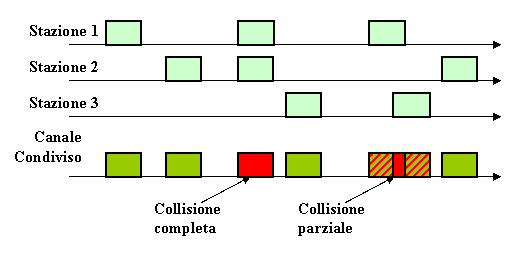
\includegraphics[scale=0.7]{res/img/22_ALOHA.png}
%\caption{Didascalia dellimmagine}
\end{figure}
\begin{figure}[H]
\centering
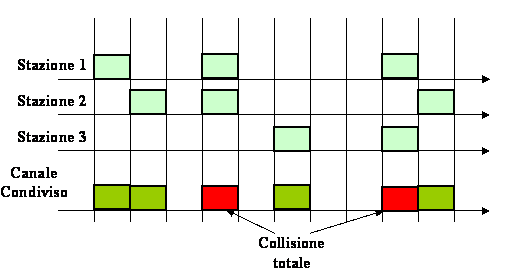
\includegraphics[scale=0.7]{res/img/22_ALOHASLOTTED.png}
%\caption{Didascalia dellimmagine}
\end{figure}

\section{Si illustri il CSMA (Carrier Sense Multiple Access), indicandone pregi e difetti}

I protocolli ALOHA e le sue varianti permettevano di inviare dati ogniqualvolta si voleva, limitando però le percentuali di successo. Per migliorare i risultati di accesso multiplo ad un mezzo di trasmissione condiviso, vengono implementati protocolli in cui le stazioni rimangono in ascolto di una portante e si comportano di conseguenza, questi protocolli sono chiamati protocolli con rilevamento della portante.
Il CSMA è una tecnica di trasmissione dati che si basa su questi principi. Ogni dispositivo prima di avviare la trasmissione dei dati deve verificare se sul canale, altri nodi stanno trasmettendo, rilevando la portante. Se il canale è libero iniziano a trasmettere, altrimenti attendono un tempo arbitrario prima di riprovare.
Esistono diverse versioni di CSMA:
\begin{itemize}
\item	CSMA 1-persistente: è il primo tra i protocolli CSMA, ha la particolarità di inviare con probabilità 1 sul canale in caso di nessun rilevamento. Questo migliora sicuramente ALOHA puro, tuttavia l’ingordigia di inviare non appena si libera il canale non rende immuni dalle collisioni, che potrebbero accadere in caso di stazioni che controllano nello stesso momento un canale vuoto e inviano contemporaneamente.
\item	CSMA non persistente: seconda variante del CSMA. Prima di trasmettere ogni stazione controlla il canale. Se lo trova libero inizia ad inviare i dati, ma se il canale è occupato la stazione non esegue un controllo continuo per trasmettere subito il proprio frame; invece attende per un intervallo casuale prima di ripetere l’algoritmo. Questo meccanismo permette di utilizzare meglio il canale ma allunga i ritardi.
\item	CSMA p-persistente: questa variante si applica su canali divisi in intervalli temporali. Quando è pronta a trasmettere, ogni stazione controlla il canale. Se lo trova libero, trasmette subito con una probabilità p, e rimanda fino all’intervallo successivo con probabilità q=1-p. Se anche quell’intervallo risulta libero la stazione trasmette oppure rimanda un’altra volta. Il processo si ripete finché il frame non è stato trasmesso.
\end{itemize}
Queste varianti migliorano enormemente il tasso di successo rispetto ad ALOHA e ALOHA-slotted.
Un ulteriore miglioramento si ottiene consentendo ad ogni stazione di annullare la propria trasmissione in caso di collisione. Se due stazioni iniziano a trasmettere contemporaneamente, invece di completare la trasmissione dei relativi frame, ormai danneggiati, terminano bruscamente la trasmissione. La terminazione rapida dei frame danneggiati risparmia tempo e banda, questa variante è chiamata CSMA/CD ed è ampiamente utilizzata nelle LAN Ethernet.

\begin{figure}[H]
\centering
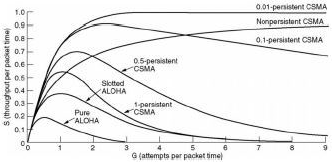
\includegraphics[scale=1]{res/img/23_CSMA.png}
%\caption{Didascalia dellimmagine}
\end{figure}

\section{Basic Bitmap}

Nella gestione di accesso multiplo ad un mezzo di trasmissione condiviso, esistono diversi protocolli che gestiscono l’accesso gestendo le collisioni e garantendo l’accesso (ALOHA, slotted ALOHA, CSMA), tuttavia le collisioni sono sfavorevoli alle prestazioni del sistema, specialmente quando il cavo è lungo e i frame corti.
Esistono però protocolli che garantiscono la gestione degli accessi senza collisione, uno tra questi è il basic Bitmap (metodo a mappa di bit elementare). In questo protocollo ogni periodo di contesa è composto esattamente da N intervalli (N=\# stazioni). Ogni stazione è numerata, e se ha un frame da inviare deve inviare un “1” nell’intervallo corrispondente al suo numero. A nessun’altra stazione è concesso di trasmettere durante questo intervallo. Cosi facendo ogni stazione si “prenota” l’intervallo di trasmissione. Una volta trascorsi gli N intervalli, ogni stazione sa quali sono le stazioni che vogliono trasmettere, di conseguenza non ci sarà mai alcuna collisione.
Questo è anche chiamato protocollo a prenotazione.
Questo protocollo non è ben bilanciato, da priorità alle stazioni con un numero basso, se una stazione “i” e una “j” vogliono trasmettere e i<j allora i si aggiudica la posizione.
Contemporaneamente però le stazioni numerate con numeri bassi dovranno attendere di più rispetto a quelle con numeri più alti.
Il basic bitmap ha bisogno di 1 bit di controllo a stazione, perciò non si adatta molto bene alle reti composte da migliaia di stazioni.

\section{Spiegare in cosa consiste il protocollo collision free binary countdown, pregi e difetti}

I dati vengono trasportati tramite un impulso elettrico. Ci possono essere molti dispositivi collegati allo stesso cavo con il rischio di collisioni e danneggiamento dei dati.
Per evitare la collisione una stazione deve controllare se ci sono altre stazioni collegate allo stesso mezzo, esistono diversi protocolli che effettuano questo controllo evitando le collisioni.
Il basic bitmap è uno di questi, tuttavia risulta elementare e su reti composte da molte stazioni risulta poco utilizzabile.
Il collision free binary countdown o conteggio binario migliora il basic bitmap, utilizzando un sistema di assegnazione della linea in base ad una stringa binaria.
Una stazione che desidera utilizzare il canale deve comunicare a tutti il proprio indirizzo sotto forma di stringa binaria, hanno tutti la stessa lunghezza.
I conflitti si evitano grazie ad una regola di arbitraggio: la stazione rinuncia ad inviare non appena si accorge che un’altra stazione con un “1” in una posizione di bit di ordine elevato che nel proprio indirizzo vale “0”.
Esempio: 0010, 0100, 1001, 1010, queste stazioni vogliono inviare, vengono inviati i primi bit: 0 (0010), 0 (0100), 1 (1001), 1 (1010), le stazioni con “0” più a sinistra capiscono che ci sono stazioni con numero più grande che stanno concorrendo e si fanno da parte, le altre due continuano: 0 (1001), 0 (1010); sono uguali quindi continuano, il terzo bit è “1” quindi la stazione 1001 si arrende, vince 1010 che può trasmettere.
L’efficienza è pari a ($d/d*log_2N$) (con d numero di bit) ma può raggiungere anche il 100\% se l’indirizzo del mittente costituisce l’intestazione del frame.
Si possono notare uno sbilanciamento notevole in quanto le stazioni con numero maggiore risultano avere sempre la precedenza, questo può essere ovviato facendo ruotare i valori delle stazioni ad ogni step, cosi quando una stazione riesce ad inviare viene spostata alla fine della coda, cosi da permettere in egual modo a tutte le stazioni la possibilità di inviare.
Questo algoritmo è semplice, elegante ed efficiente, tuttavia attualmente non è utilizzato.

\begin{figure}[H]
\centering
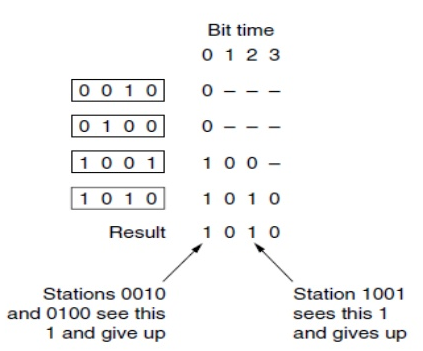
\includegraphics[scale=0.6]{res/img/25_FreeBinaryCountdown.png}
%\caption{Didascalia dellimmagine}
\end{figure} 

\section{Spiegare cos’è l’adaptive tree walk protocol?}

Per gestire la contesa di accesso ad un canale condiviso esistono protocolli con controllo della portante, con metodo della contesa tipo il CSMA o il metodo senza collisioni. Nelle situazioni di carico leggero la contesa è preferibile per il suo basso ritardo, tuttavia a carichi elevati diventa sempre più inefficiente. Il contrario avviene con i protocolli senza collisioni, a basso carico hanno un ritardo elevato ma al crescere del carico l’efficienza migliora.
Adaptive tree walk protocol è un protocollo a contesa limitata che migliora ulteriormente le prestazioni dei protocolli sopracitati.
Si può immaginare questo metodo come un albero binario, in cui le stazioni sono le foglie e sono divise nei vari rami. Inizialmente si prova a inviare ad altezza 0 se non vi è collisione si procede all’invio, in caso contrario ci si sposta sul sottoalbero sinistro e si ritenta, se il conflitto non c’è più si fa inviare la stazione che lo desidera (se non c’è conflitto vuol dire che nel sottoalbero sinistro c’è solo una stazione che vuole inviare). Dopo aver inviato si torna al nodo padre e si analizza il sottoalbero destro, ripetendo i test e scendendo nei sottoalberi in caso di conflitto.

\begin{figure}[H]
\centering
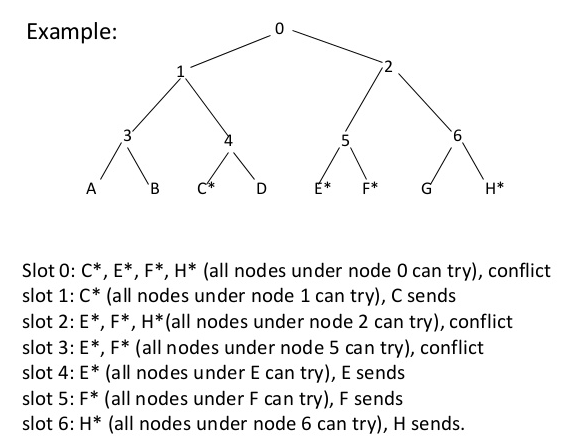
\includegraphics[scale=0.7]{res/img/26_AdaptiveTreeProtocol.png}
%\caption{Didascalia dellimmagine}
\end{figure}
 
\section{Ethernet e i vari tipi di cavo}

Ethernet è il sistema LAN più diffuso al mondo, è economico e facile da usare e la diffusione delle componenti hardware ne ha facilitato l’adozione, è adeguata all’utilizzo con TCP/IP.
Nasce con l’intento di ottenere una trasmissione affidabile su cavo coassiale in condizioni di traffico contenuto, ma in grado di tollerare possibili picchi di carico. Per regolamentare l’accesso al mezzo trasmissivo era stato adottato un protocollo di accesso multiplo del tipo CSMA/CD.
Il nome Ethernet si riferisce al cavo (definito “etere”), andiamo quindi ad elencare le tipologie di cavi utilizzati in questo standard.
Generalmente vengono utilizzati 4 tipi di cavo, il più vecchio è il modello 10base5 chiamato anche thick Ethernet, questo cavo assomiglia ad un tubo giallo con segni a intervalli di 2,5m che indicano la posizione delle spine.
Le connessioni sono generalmente realizzate mediante spine a vampiro (spilli spinti nel nucleo centrale del cavo coassiale). 
La notazione 10Base5 indica che opera a 10Mbps, utilizza un sistema di segnali a banda base e può supportare segmenti lunghi fino a 500m. Questo cavo è ormai obsoleto.
Il secondo cavo in ordine di tempo è stato il cavo 10base2 o thin Ethernet, più facile da piegare rispetto al precedente e le connessioni sono realizzate usando connettori BNC (giunzioni a “T” più affidabili e facili da usare rispetto alle spine a vampiro.). Il thin Ethernet è più economico e semplice da installare, però può essere lungo al massimo 185 metri e può supportare non più di 30 macchine.
Per trovare guasti in questi mezzi è usata la tecnica TDR (Time Domain Rectory) che sostanzialmente misura il ritardo dell'eco dell'impulso immesso nel cavo.
La tecnica TDR per la ricerca di guasti è difficile e onerosa da utilizzare, ci si è spostati quindi sulla terza tipologia di cablaggio 10Base-T, ormai diventata uno standard grazie alla facilità di gestione e all’uso di cablaggi preesistenti.
Questo sistema di cablaggio utilizza hub di controllo tramite doppini telefonici, che sono largamente usati e semplici da gestire, ogni macchina si interfaccia con l’hub tramite cavo dedicato; rendendo cosi semplice aggiungere o rimuovere una stazione e individuare le interruzioni. Il suo svantaggio è rappresentato dalla lunghezza massima dei cavi che partono dall’hub: 100 metri. Esiste una versione più veloce del 10Base-T chiamata 100Base-T.
Il quarto tipo di cavi per Ethernet si chiama 10Base-F e utilizza le fibre ottiche. È un’alternativa costosa a causa del prezzo dei connettori e dei terminatori, ma offre un’eccellente immunità alle interferenze e consente di collegare edifici o hub molto lontani. 10Base-F nonostante il costo consente inoltre una buona sicurezza in quanto i dati trasmessi sulla fibra sono difficili da intercettare.
 
\begin{figure}[H]
\centering
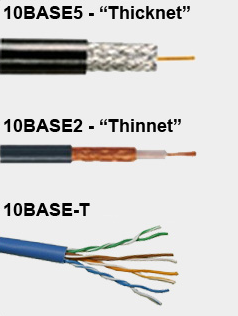
\includegraphics[scale=0.6]{res/img/27_CaviEthernet.png}
%\caption{Didascalia dellimmagine}
\end{figure}

\section{Codifica Manchester}

Nel sistema Ethernet la codifica binaria del segnale è “0” viene indicato con 0 volt mentre “1” utilizzando 5 volt, questo fa sorgere numerosi problemi, in quanto altre stazioni potrebbero interpretare erroneamente il segnale (a causa degli 0 volt, una stazione potrebbe confondere l’assenza del segnale con uno “0”). Si può passare a +1 volt per “1” e -1 volt per “0”, ma rimane il problema dei ricevitori che possono campionare il segnale in maniera diversa.
Per risolvere questo problema sono state inventate due tecniche codifica Manchester e codifica Manchester differenziale.
Queste codifiche sono dette auto-sincronizzanti in quanto non necessitano di un segnale di sincronia esterno.
Queste codifiche suddividono ogni bit codificato in due, nella codifica Manchester lo “0” viene rappresentato da un segnale Basso-Alto, mentre l’”1” viene rappresentato da un segnale Alto-Basso. (esistono due convenzioni opposte riguardo la rappresentazione dei segnali “1” e “0”).
Cosi facendo anche in caso di dissincronia, i dati in questo formato permettono un flusso auto-sincronizzante.
La codifica Manchester differenziale invece differisce da quella originale nella rappresentazione dei bit: questa infatti si basa sulla verifica di transizioni all’inizio di un intervallo. La presenza di una di queste infatti (che siano alto-basso o basso-alto) identifica un valore, la mancanza di transizione invece indica il valore opposto. Per convenzione il bit 1 viene rappresentato dalla mancanza di transizione all’inizio del suo intervallo, mentre lo 0 è indicato con un cambiamento di segnale nello stesso periodo.
Tutti i sistemi Ethernet adottano la codifica Manchester perché è più semplice, mentre la Manchester differenziale è utilizzata da altre LAN.

\begin{figure}[H]
\centering
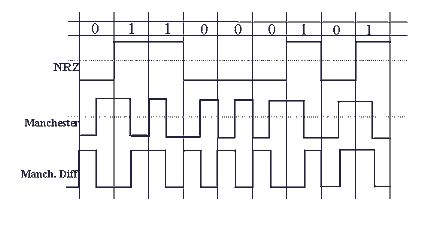
\includegraphics[scale=0.8]{res/img/28_CodificaManchester.png}
%\caption{Didascalia dellimmagine}
\end{figure}
 
\section{Cos’è il binary exponential backoff?}

Nel protocollo di accesso multiplo CSMA/CD viene utilizzato l’algoritmo di backoff esponenziale, il quale serve a decidere il tempo di entrata di una stazione nel canale dopo aver riscontrato una collisione.
La caratteristica principale del CSMA/CD (algoritmo che controlla il canale prima di trasmettere ed evita le collisioni analizzando la portante) è che una volta rilevata una collisione, si attende un intervallo prima di ritrasmettere, questo intervallo viene calcolato ogni volta tramite l’algoritmo di backoff esponenziale.
Dopo una collisione il tempo viene diviso in intervalli discreti, la cui lunghezza è uguale al tempo di propagazione di andata e ritorno del caso peggiore sul mezzo di trasmissione.
Dopo la prima collisione, ogni stazione aspetta 0 o 1 intervalli temporali prima di ritentare. Se due stazioni collidono e ognuna sceglie lo stesso numero casuale, la collisione si ripeterà. Dopo la seconda collisione ogni stazione sceglie 0, 1, 2 o 3 a caso e rimane in attesa per quel numero di intervalli temporali. In generale quindi, dopo i collisioni, viene scelto un numero casuale compreso tra 0 e 2i-1 e si salta quel numero di intervalli. Il limite di collisioni è 16, dopodiché il chip di controllo getta la spugna e manda un errore.
Questo algoritmo è stato scelto perché si adatta dinamicamente al numero di stazioni che tentano di trasmettere. Poiché l’intervallo di scelta casuale cresce esponenzialmente con il numero di collisioni avvenute l’algoritmo assicura un basso ritardo quando poche stazioni collidono e garantisce un intervallo di tempo ragionevole quando la collisione coinvolge molte stazioni.




\section{Stazione nascosta e stazione esposta: cosa sono e cosa fanno?}

Al crescere del numero di computer e dispositivi mobili aumenta anche la domanda di collegare tali apparecchi al mondo esterno.
Nascono così le LAN wireless, le quali permettono la connessione dei dispositivi senza bisogno di cavi.
Tuttavia, questo porta a dei problemi di conflitto in caso di scambio di dati.
Utilizzando banalmente il sistema CSMA per evitare le collisioni, porterebbe ad ascoltare le altre trasmissioni, e trasmettere in caso di nessun’altra connessione attiva.
Questo però può portare a due diversi problemi: problema della stazione nascosta e stazione esposta.
La stazione nascosta non è altro che una stazione che vuole inviare, non riesce a ricevere i segnali dei concorrenti a causa della sua distanza eccessiva. Supponiamo di avere A, B e C. A vuole inviare a B, prima di farlo ascolta se ci sono altre connessioni, non ne sente e procede all’invio. Tuttavia, C, è troppo distante perché A lo senta, ma abbastanza vicino a B per inviargli dati, cosi lo fa e va in conflitto con l’invio di A.

\begin{figure}[H]
\centering
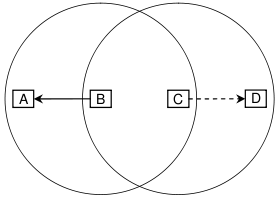
\includegraphics[scale=0.6]{res/img/30_StazioneEsposta.png}
%\caption{Didascalia dellimmagine}
\end{figure} 
 
Il problema della stazione esposta invece è l’inverso, B trasmette ad A, C vuole inviare a D e controlla la presenza di portante sul mezzo di trasmissione e rileva B che sta inviando, cosi attende per evitare conflitti, tuttavia B non intralcerebbe la trasmissione di C, ma questo non lo può sapere, di conseguenza si genera uno stallo inutile. Questo è il problema della stazione esposta.
 
 \begin{figure}[H]
\centering
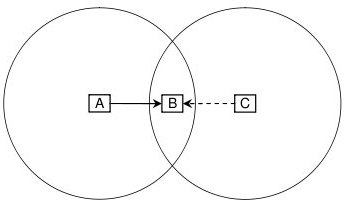
\includegraphics[scale=0.6]{res/img/30_StazioneNascosta.png}
%\caption{Didascalia dellimmagine}
\end{figure} 
\section{Bluetooth}
\subsection{Cos'è?}
Bluetooth è uno standard wireless che permette il collegamento di dispositivi di calcolo, di comunicazione e accessori vari mediante un sistema radio wireless a basso costo, bassa potenza e portata ridotta.

L’unità di base di un sistema Bluetooth è la piconet, composta da un nodo master e da diversi nodi slave (non più di 7), situati nel raggio di 10 metri. Più piconet possono trovarsi nella stessa stanza e possono essere collegate tramite un nodo ponte; un insieme di piconet è chiamato scatternet.

Tutto si basa sulla comunicazione tra nodo master e nodo slave. Il master controlla il clock e decide quale dispositivo può comunicare in ogni intervallo temporale.

I tipi di collegamenti si suddividono in due tipi principali: orientati alla connessione o senza connessione.
Il primo richiede di stabilire una connessione tra i dispositivi prima di inviare i dati, mentre in quello senza connessione il trasmettitore può in qualsiasi momento iniziare a inviare i propri pacchetti purché conosca l’indirizzo del destinatario.

Bluetooth definisce inoltre due tipi di collegamenti a supporto delle applicazioni voce e trasferimento dati: un servizio asincrono senza connessione (ACL) ed un servizio sincrono orientato alla connessione (SCO).
ACL supporta il traffico dati e si basa su un servizio di tipo best-effort (ovvero un servizio che non dà alcuna garanzia dell’effettiva consegna dei dati né tantomeno livelli di qualità o priorità garantiti).
Supporta connessioni a commutazione di pacchetto, connessioni punto-multipunto (multicast) e connessioni simmetriche o asimmetriche.
SCO invece è un collegamento che supporta connessioni con un traffico di tipo real-time e multimediali, prevede connessioni a commutazione di circuito, connessioni punto-punto e connessioni simmetriche.

Bluetooth ha protocolli raggruppati in strati, che non seguono ne modello OSI né TCP/IP.

\section{Si descriva l’algoritmo statico Flooding}

La funzione principale dello strato network è quella d’instradare i pacchetti dal computer sorgente al computer di destinazione.
Lo strato network sfrutta particolari algoritmi detti algoritmi di routing per instradare correttamente i pacchetti nei vari percorsi. Esistono diversi modi per farlo, in quanto ci sono molti fattori da tenere in considerazione, però possiamo suddividerli in due grandi tipi: algoritmi non adattivi e algoritmi adattivi.

Gli algoritmi non adattivi basano le loro decisioni su misure e stime del traffico e della topologia corrente, viene calcolato il percorso all’avvio della rete, in modalità fuori linea e viene scaricato nei router. Questa procedura si chiama anche routing statico. Gli algoritmi adattivi invece cambiano le loro decisioni secondo le modifiche apportate alla topologia e al traffico.
\subsection{Cos'è?}
L’algoritmo di Flooding è un algoritmo statico, in cui ogni pacchetto in arrivo è inviato a tutte le linee tranne quella da cui proviene.

Una variante un po’ più pratica è chiamata flooding selettivo. In questo algoritmo i router non trasmettono ogni pacchetto verso tutte le linee, ma solo attraverso quelle che vanno approssimativamente nella direzione corretta.
Nella maggior parte delle applicazioni questo algoritmo non è molto utilizzato, salvo casi particolari (i militari lo utilizzano, in quanto un gran numero di router potrebbero saltare in aria, aver questo metodo di trasmissione di pacchetti accerta la ricezione dei dati).

Questo algoritmo viene utilizzato anche come metrica di confronto per altri algoritmi di routing, in quanto sceglie sempre il percorso più breve (scegliendoli tutti LOL), di conseguenza nessun algoritmo può produrre un ritardo più breve (ignorando il tempo di elaborazione dati generato dal processo di flooding).

\begin{figure}[H]
\centering
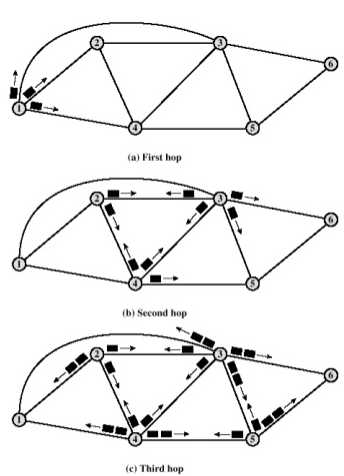
\includegraphics[scale=0.7]{res/img/32_Flooding.png}
\end{figure}

\subsection{Pregi}
Semplice da attuare e assicura la ricezione del pacchetto alla stazione desiderata.

\subsection{Difetti}
Spreco evidente di banda, pacchetti duplicati e rischio di cicli infiniti.

\subsection{Ambiti d'uso}
Strato Network.
Questo algoritmo viene utilizzato come metrica di confronto per altri algoritmi di routing, in quanto sceglie sempre il percorso più breve (tra i molteplici).
Utilizzato anche in ambito militare in quanto la duplicazione dei pacchetti può essere una nota positiva a causa del rischio di bombardamenti.

\section{Descrivere il distance vector routing}

La funzione principale dello strato network è quella d’instradare i pacchetti dal computer sorgente al computer di destinazione. Per fare questo vengono utilizzati diversi algoritmi che si possono raggruppare in due grandi gruppi: algoritmi adattivi e non adattivi. Gli algoritmi non adattivi sono anche detti statici, in quanto basano i loro calcoli sulla rete “a freddo” senza tener conto del carico istantaneo o dei problemi di linea; un esempio è l’algoritmo di Flooding.

Generalmente le moderne reti di computer utilizzano algoritmi adattivi, o dinamici se vogliamo. Tra i più popolari ci sono il distance vector routing e il linkstate routing.
\subsection{Cos'è?}
Gli algoritmi di routing basati sul vettore delle distanze (distance vector routing) operano facendo in modo che ogni router conservi una tabella (vettore) che definisce la miglior distanza conosciuta per ogni destinazione e la linea che lo conduce ad essa. Queste tabelle vengono aggiornate scambiando informazioni con i router vicini.

Questo algoritmo è basato sull’algoritmo di Bellman-Ford (che calcola i cammini minimi su un grafo).
Ogni router misura la “distanza” (secondo una metrica che può includere vari fattori) che lo separa dai nodi adiacenti ricevendo i dati dai router vicini. A partire da tali dati, utilizzando l’algoritmo di Bellman-Ford, il router costruisce una tabella che associa ad ogni destinazione conosciuta la stima della distanza che lo separa dalla destinazione e il primo passo del percorso calcolato.
Questo aggiornamento viene fatto periodicamente e dopo sufficienti scambi ciascun router avrà una riga per ogni altro nodo nella rete.

\begin{figure}[H]
\centering
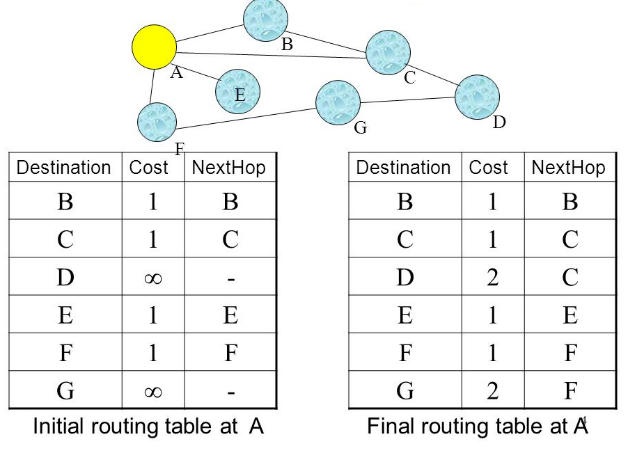
\includegraphics[scale=0.8]{res/img/33_DistanceVectorRouting.png}
\end{figure} 


\subsection{Pregi}
Ogni router ha il percorso migliore per arrivare a tutti i suoi nodi adiacenti.

\subsection{Difetti}
Impiega troppo tempo a raggiungere la convergenza.\\
Non tiene conto della banda della linea quando sceglie i percorsi.\\
Possibilità che si creino i cicli, potenzialmente infiniti.

\subsection{Ambiti d'uso}
Strato network per instradare i pacchetti ai vari router della rete, algoritmo adattivo (dinamico).

\section{Descrivere Linkstate routing}

La funzione principale dello strato network è quella d’instradare i pacchetti dal computer sorgente al computer di destinazione. Per fare questo vengono utilizzati diversi algoritmi che si possono raggruppare in due grandi gruppo: algoritmi adattivi e non adattivi. Gli algoritmi non adattivi sono anche detti statici, in quanto basano i loro calcoli sulla rete “a freddo” senza tener conto del carico istantaneo o dei problemi di linea; un esempio è l’algoritmo di Flooding.

Generalmente le moderne reti di computer utilizzano algoritmi adattivi, o dinamici se vogliamo. Tra i più popolari ci sono il distance vector routing e il linkstate routing.
\subsection{Cos'è?}
Gli algoritmi di routing basati sullo stato dei collegamenti (linkstate routing) è il sostituto del distance vector routing. L’idea di questo algoritmo si basa su 5 punti:
\begin{itemize}
\item	Scoprire i propri vicini e i relativi indirizzi di rete.
\item	Misurare il ritardo o il costo di ogni vicino.
\item	Costruire un pacchetto che contiene tutte le informazioni raccolte.
\item	Inviare questo pacchetto a tutti gli altri router
\item	Elaborare il percorso più breve verso gli altri router.
\end{itemize}

Un router, prima di tutto, cerca di scoprire chi sono i suoi vicini: lo fa inviando uno speciale pacchetto “HELLO” su ogni linea punto-punto; il router all’altro capo risponde fornendo la propria identità (si noti che i nomi devono essere globalmente unici, in quanto si necessità una non ambiguità durante lo scambio di pacchetti).

Il passo successivo è la misurazione del costo della linea, avviene tramite l’invio di uno speciale pacchetto “ECHO” al quale l’altra parte deve rispondere immediatamente, in base al tempo di andata/ritorno si può ottenere una stima ragionevole del ritardo.

Dopo aver raccolto le informazioni necessarie per lo scambio, ogni router deve costruire un pacchetto contenente tutti i dati. Il pacchetto inizia con l’identità del trasmittente, un numero di sequenza, l’età (contatore che viene decrementato ogni secondo, al raggiungere dello 0 le informazioni provenienti da quel router vengono scartate) e una lista dei vicini. Per ogni vicino è riportato il ritardo misurato. I pacchetti vengono creati periodicamente, oppure in caso di avvenimenti speciali: interruzione della linea o modifica/spegnimento/accensione di un vicino.

La parte più delicata dell’algoritmo è la distribuzione affidabile dei pacchetti che contengono la descrizione dello stato dei collegamenti. Durante la distribuzione e l’installazione, i router che ricevono i primi pacchetti cambieranno i loro percorsi, rischiando di creare inconsistenza, cicli, computer irraggiungibili e così via. L’idea fondamentale è quella di utilizzare l’algoritmo di flooding (inviare ogni pacchetto ad ogni linea in uscita (tranne da dov’è arrivato)) un computer che riceve un pacchetto con le informazioni sullo stato della connessione:
\begin{itemize}
\item	Se è duplicato il pacchetto viene scartato
\item	Se è nuovo il pacchetto viene inoltrato a tutte le linee tranne a quella di ricezione (flooding)
\item	Se il numero di sequenza è inferiore al numero più alto visto in quel momento, il pacchetto viene scartato in quanto obsoleto (il router ha informazioni più recenti).
\end{itemize}
Esistono diversi miglioramenti per questo metodo di distribuzione di pacchetti, ma sarebbe troppo lunga da elencare.

Dopo aver accumulato una serie completa di pacchetti sullo stato della connessione, il router può costruire l’intero grafo della sottorete, lo fa utilizzando localmente l’algoritmo di Dijkstra (algoritmo per la costruzione di grafi, simile a quello di Bellman-Ford, non può essere però utilizzato in caso di cammini negativi).

Questo algoritmo è molto utilizzato nelle reti reali in quanto può gestire reti composte da molti nodi, converge rapidamente al cammino minimo, difficilmente genera cicli ed è facile da comprendere in quanto ogni nodo ha la mappa completa della rete. Il principale svantaggio è la complessità di realizzazione, anche dovuta alla notevole capacità di memoria ed elaborazione richiesti dai router.

\subsection{Pregi}
Può gestire reti molto caotiche.\\
Converge velocemente al cammino minimo.\\
Difficilmente genera cicli.\\
Facile da comprendere.

\subsection{Difetti}
Difficile da realizzare, a causa della notevole capacità di memoria ed elaborazione richiesta dai router.

\subsection{Ambiti d'uso}
Strato network, sostituto al distance vector routing.
Molto utilizzato nelle reti attuali visti i numerosi pregi.

\section{Choke packet}

La funzione principale dello strato network è quella d’instradare i pacchetti dal computer sorgente al computer di destinazione. La decisione del miglior percorso viene effettuato dagli algoritmi di routing (flooding, linkstate o distance vector). Purtroppo, per molteplici motivi, le reti potrebbero congestionarsi, più computer vogliono inviare pacchetti alla stessa destinazione che, non riuscendo ad elaborarli tutti ne perde, questo causa la ritrasmissione che causa ulteriori ingorghi. Questo problema è la congestione ed è un punto critico che va regolamentato.
\subsection{Cos'è?}
Il choke packet è uno speciale pacchetto utilizzato per il controllo di flusso in una rete. Un router che rileva una congestione, invia all’host originale del pacchetto un choke packet per avvertirlo di diminuire il flusso. Quando l’host sorgente riceve il pacchetto speciale diminuisce il flusso (tipicamente lo dimezza) e ignora i successivi choke packet (generalmente ne arrivano in rapida successione), passato un tempo prefissato l’host si rimette all’ascolto, se arrivano altri choke packet in quel frangente diminuisce ulteriormente il flusso, altrimenti riprende gradualmente la velocità normale.

\begin{figure}[H]
\centering
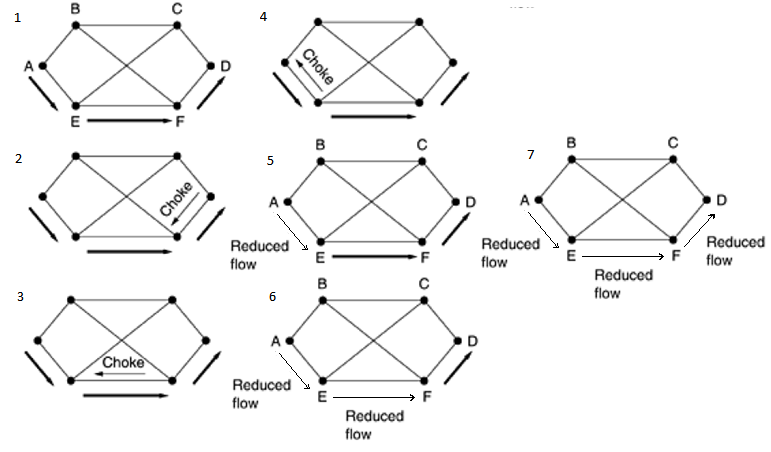
\includegraphics[scale=0.6]{res/img/35_ChokePacket.png}
\end{figure}
\subsection{Pregi}
Permette di risolvere la congestione di una linea tramite l'uso di uno speciale pacchetto.

\subsection{Difetti}
Lento a reagire, purtroppo l'host produttore di pacchetti che genera la congestione, ci mette un certo tempo per ricevere il choke packet e prendere provvedimenti. Un miglioramento si ha con il Choke packet hop-by-hop (altro algoritmo per risolvere la congestione).

\subsection{Ambiti d'uso}
Strato network, algoritmo di controllo della congestione.

\section{Choke packet hop-by-hop}

La funzione principale dello strato network è quella d’instradare i pacchetti dal computer sorgente al computer di destinazione. La decisione del miglior percorso viene effettuato dagli algoritmi di routing (flooding, linkstate o distance vector). Purtroppo, per molteplici motivi, le reti potrebbero congestionarsi, più computer vogliono inviare pacchetti alla stessa destinazione che, non riuscendo ad elaborarli tutti ne perde, questo causa la ritrasmissione che causa ulteriori ingorghi. Questo problema è la congestione ed è un punto critico che va regolamentato.
\subsection{Cos'è?}
Il hop-by-hop choke packet è un miglioramento della sua versione precedente (choke packet).
Choke packet aveva il problema di aver un tempo di reazione per prendere provvedimenti troppo lento, il che causava una grossa perdita di dati prima di risolvere il problema.

Hop-by-hop choke packet risolve questo problema limitando tutte le stazioni che attraversa in maniera immediata, senza dover attendere di arrivare all’host sorgente.


\begin{figure}[H]
\centering
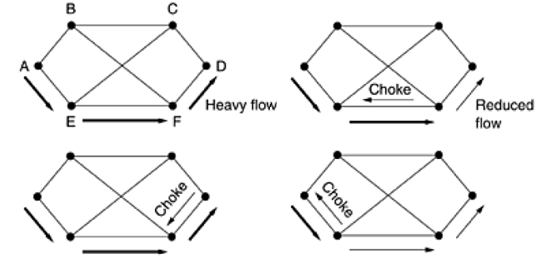
\includegraphics[scale=0.6]{res/img/36_ChokePacketHopbHop.png}
\end{figure}
 
\subsection{Pregi}
Rispetto al choke packet originale, da sollievo più veloce alla rete.
\subsection{Difetti}
Richiede maggior utilizzo dei buffer di trasmissione nei router tra mittente e destinatario.
\subsection{Ambiti d'uso}
Strato network, algoritmo di controllo della congestione, miglioramento del choke packet.

\section{Load shedding}
La funzione principale dello strato network è quella d’instradare i pacchetti dal computer sorgente al computer di destinazione. La decisione del miglior percorso viene effettuato dagli algoritmi di routing (flooding, linkstate o distance vector). Purtroppo, per molteplici motivi, le reti potrebbero congestionarsi, più computer vogliono inviare pacchetti alla stessa destinazione che, non riuscendo ad elaborarli tutti ne perde, questo causa la ritrasmissione che causa ulteriori ingorghi. Questo problema è la congestione ed è un punto critico che va regolamentato.
\subsection{Cos'è?}
Quando gli algoritmi di choke packet (puro e hop-by-hop) non bastano per gestire la congestione, i router possono utilizzare la tecnica load shedding che, molto banalmente elimina dei pacchetti casuali in caso di sovraffollamento.

Lo scartare pacchetti casuali non è sempre la scelta migliore, per migliorare l’algoritmo infatti la scelta può basarsi sull’applicazione in esecuzione. Esistono due criteri generali per identificare queste scelte, wine e milk.

Wine da più importanza ai pacchetti vecchi, scarta di conseguenza quelli nuovi (vecchio è meglio del nuovo), milk invece al contrario dà importanza maggiore ai pacchetti nuovi (nuovo è migliore del vecchio).

Questa tecnica permette numerose applicazioni e metodi per implementarla (oltre a wine e milk). Questo permette di tenere sotto controllo possibili momenti di congestione.

\subsection{Pregi}
Risolve la congestione in modo brutale, quando il choke packet non basta.

\subsection{Difetti}
Scarta pacchetti senza un criterio sufficientemente preciso da evitare di scartare pacchetti importanti.

\subsection{Ambiti d'uso}
Strato network, metodo brutale utilizzato per risolvere la congestione delle linee.

\section{Red (Random Early Detection)}

Nello strato network esistono numerosi algoritmi di instradamento per portare un pacchetto da una destinazione ad un mittente (flooding, distance vector, linkstate). Quando questa linea si congestiona esistono algoritmi che permettono di gestire la congestione e risolvere il problema (choke packet e load shedding). Risulta tuttavia più semplice gestire la congestione appena viene rilevata, non cercare di porvi rimedio dopo averle dato il tempo di bloccare tutta la linea.
\subsection{Cos'è?}
Questa osservazione porta all’idea di scartare i pacchetti prima che il buffer sia completamente pieno. Da qui nasce un celebre algoritmo usato per mettere in pratica questo schema: \textbf{RED} (Random Early Detection).

Red fa in modo che i router scartino i pacchetti prima che la situazione diventi senza speranza (early). Per stabilire quando è il momento giusto per iniziare a scartare i pacchetti, i router mantengono una media mobile delle lunghezze delle code. Quando la lunghezza media su una linea supera una soglia di guardia allora quella determinata linea è considerata congestionata e prende le dovute azioni di correzione. Il massimo che può fare purtroppo è scegliere un pacchetto a caso dalla coda che ha attivato “l’azione difensiva” e scartarlo. Per segnalare il rischio di congestione il router potrebbe inviare un choke packet per chiedere la diminuzione di flusso, tuttavia questo congestionerebbe ulteriormente le linee.

Scartando il pacchetto, la sorgente lo invierà nuovamente a causa del mancato acknowledgement.

\subsection{Pregi}
Risolve le congestioni prima che sia troppo tardi e sia necessario scartare pacchetti con il load shedding.

\subsection{Difetti}
Non può sapere esattamente che pacchetto ha causato il superamento della soglia (di conseguenza non sa chi è il reale mittente), di conseguenza non è il massimo della precisione.

\subsection{Ambiti d'uso}
Viene utilizzato prevalentemente nelle reti in cui le sorgenti rispondono ai pacchetti perduti rallentando il flusso.\\
Nelle reti wireless la perdita dei pacchetti è causata dal rumore nella maggior parte dei casi, di conseguenza non si rallenta il flusso e RED è impossibile da utilizzare.

\section{Reverse Path Forwarding}

I router spesso necessitano di inviare messaggi a molti o a tutti gli altri host. Questi tipi di trasmissioni sono dette trasmissioni broadcast.

L’algoritmo di routing più quotato per questo genere di trasmissioni è sicuramente quello di flooding, in quanto invia i pacchetti a tutte le stazioni vicine (tranne quella da cui ha ricevuto il pacchetto). Un problema di questa tecnica è sicuramente lo spreco di banda e la creazione di troppi pacchetti.
Per ovviare a questo problema sono stati creati numerosi algoritmi che cercano di migliorare questo sistema di broadcasting.

\subsection{Cos'è?}
Con il Reverse path forwarding, il router che riceve un pacchetto controlla se gli è giunto da una linea che normalmente è utilizzata per inviare i pacchetti alla sorgente (ovvero che sia la linea con cammino minimo da lui alla sorgente). In caso affermativo, c’è una forte probabilità che il pacchetto broadcast abbia seguito il percorso migliore dalla sorgente fino a lui, di conseguenza lo copia e lo inoltra a tutte le linee (tranne quella da cui l’ha ricevuto). Se invece il pacchetto broadcast è giunto attraverso una linea diversa dalla preferita per raggiungere la sorgente, il pacchetto viene scartato in quanto è probabile si tratti di un duplicato.


\subsection{Pregi}
Implementazione facile ed efficiente: non richiede di conoscere la mappa della sottorete, liste di destinazione o mappe di bit per ogni pacchetto.\\
Previene il problema dell'IP spoofing (falsificazione dell'indirizzo del mittente).
\subsection{Difetti}
--
\subsection{Ambiti d'uso}
Strato Network, tecnica usata nei moderni router con lo scopo di assicurare un cammino di pacchetti privi di loop.

\section{Quality of Service (QoS)}

Un flusso di pacchetti da una sorgente a una destinazione è chiamato, appunto, flusso.
Ogni flusso viene regolamentato per il percorso da effettuare e quando effettuarlo, i metodi di gestione della congestione e così via.
\subsection{Cos'è?}
Ogni flusso ha le sue esigenze, in base all’applicazione che sta servendo, possiamo quindi caratterizzare queste esigenze in quattro parametri primari: affidabilità, ritardo, jitter e banda. Insieme, questi parametri determinano la QoS (Quality of Service), ossia la qualità del servizio richiesta dal flusso.
\begin{itemize}
\item	\textbf{Affidabilità}: nessun bit può essere trasmesso in modo scorretto. Questo obiettivo viene di solito raggiunto creando il checksum di ogni pacchetto e verificandolo alla destinazione. Questo parametro è ricercato da applicazioni tipo la posta elettronica o trasferimento di file, che necessitano di un’alta affidabilità, applicazioni come audio o video possono tollerare errori, perciò non viene elaborato o verificato nessun checksum.
\item	\textbf{Ritardo}: il ritardo dei pacchetti in applicazioni come la posta elettronica o il trasferimento file non è molto sentito, è importante invece in applicazioni come telefonate o videoconferenze.
\item	\textbf{Jitter}: Il Jitter non è altro che la variazione del segnale in modo casuale. Questo può portare ad una ricezione di dati in intervalli irregolari, applicazioni come può essere la posta elettronica o il trasferimento file non sono molto soggette a questo problema. Lo sono invece per applicazioni di login remoto o di streaming video, a causa della variazione casuale della trasmissione, il risultato è terribile.
\item	\textbf{Banda}: ogni applicazione differisce per l’esigenza di banda, posta elettronica e accesso remoto non ne richiede molta, il video in tutte le sue forme invece sì.
\end{itemize}
Nessuna tecnica è in grado di fornire QoS efficiente e sicura in modo ottimo. 

\begin{figure}[H]
\centering
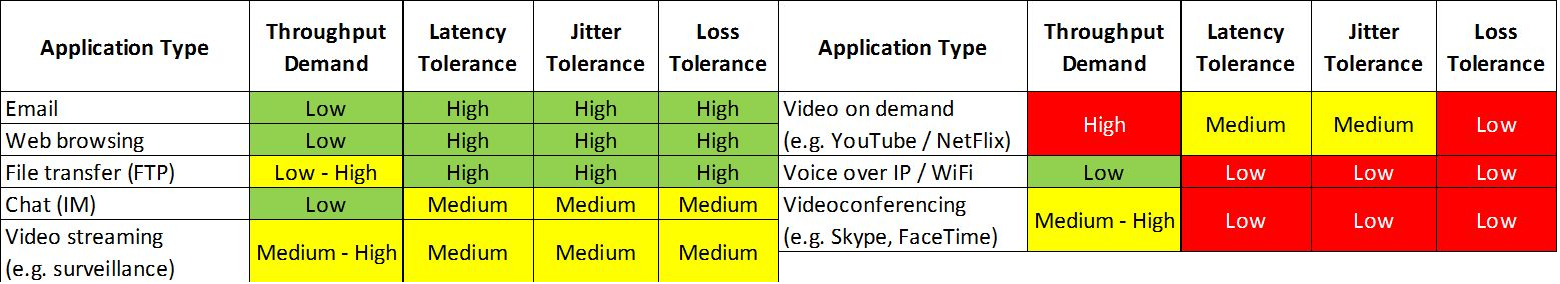
\includegraphics[scale=0.3]{res/img/40_QoS.png}
\end{figure}
\section{Leaky bucket, pregi e difetti}

Quando ci si scambia pacchetti nella rete, serve un modo per controllare il flusso; per delimitare banda e velocità di trasmissione si può utilizzare l’algoritmo leaky bucket, un sistema di accodamento a singolo server con tempo di servizio costante.

Questo algoritmo si basa sull’idea del “secchio che perde” attraverso il quale qualsiasi quantità d’acqua contenuta fluirà all’esterno sempre con la stessa velocità, se l’acqua viene aggiunta troppo velocemente questa supererà in volume la capacità del secchio e straborderà.

Allo stesso modo il leaky bucket è formato da una coda finita. Al suo arrivo, se c’è spazio il pacchetto viene aggiunto alla coda, altrimenti viene scartato. Ad ogni ciclo di clock viene trasmesso un pacchetto (se la coda non è vuota).

Così facendo si gestiscono burst di dati che altrimenti congestionerebbero la rete; un contro però può essere che, siccome trasmette pacchetti solo ad intervalli prefissati, ci saranno parecchi casi in cui il volume del traffico sarà molto basso e ampie porzioni di risorse di rete non verranno utilizzate.

\section{Descrivere il token bucket, pregi e difetti}

Per gestire il flusso di pacchetti su una rete è necessario utilizzare algoritmi che permettano un controllo della congestione e che sfruttino al meglio le risorse di rete. L’algoritmo leaky bucket (secchio che perde) gestiva le congestioni, ma purtroppo imponeva un modello di output troppo rigido, che non seguiva la variabilità del traffico.

Per molte applicazioni è meglio permettere all’output di accelerare un po’ quando ci sono burst di dati, perciò serve un algoritmo più flessibile e che non perda mai dati.

L’algoritmo token bucket riprende l’idea del leaky bucket, ma aggiunge dei token, generati da un clock.
Un pacchetto per passare deve distruggere un token, se non c’è attende finché non viene generato dal clock. A differenza del leaky bucket, il token bucket non scarta i pacchetti quando il secchio è pieno.

Se non arrivano pacchetti da inviare, il token bucket accumula i token fino ad un massimo di n. Così facendo si prepara a gestire dei possibili burst di massimo n pacchetti (pari al numero di token), bruciando i token in rapida successione e dando una risposta più veloce a picchi improvvisi.

Per implementare questo algoritmo è necessaria solo una variabile che tenga conto del numero di token, e li diminuisca quando un pacchetto viene inviato.
 
\section{Descrivere l’ARP}
Ogni macchina di Internet ha uno o più indirizzi IP, tuttavia questi non possono essere utilizzati per inviare pacchetti, in quanto l’hardware che opera sullo strato data link non comprende gli indirizzi Internet.
Bisogna trovare un modo per associare l’indirizzo Ethernet a 48 bit (indirizzo MAC) con l’indirizzo IP associato.

ARP è un protocollo che permette di associare ad un indirizzo IP all’indirizzo Ethernet in una sottorete (o anche tra più sottoreti utilizzando Arp-proxy).
Viene trasmesso un pacchetto broadcast a tutte le stazioni nella sottorete che chiede chi è il proprietario di un determinato indirizzo IP. Le stazioni controllano il proprio indirizzo IP e solo il proprietario di tale indirizzo risponde inviando il proprio indirizzo Ethernet. In questo modo la stazione che cercava un determinato indirizzo riesce a collegare l’IP con il MAC.

A questo punto, il software IP costruisce un frame Ethernet indirizzato al destinatario appena scoperto e inserisce il pacchetto IP nel campo carico utile, dopodiché scarica tutto sulla Ethernet. 
La scheda Ethernet del destinatario rileva il frame, si accorge di essere la stazione designata della comunicazione, preleva i dati ed estrae il pacchetto IP dal carico utile per passarlo al software IP, il quale verifica la correttezza dell’indirizzo ed elabora i dati.
Per migliorare le prestazioni, dopo aver associato degli indirizzi, questi vengono memorizzati nella cache, cosi, in caso di nuove trasmissioni verso la stessa stazione, si ha già l’indirizzo pronto.

Questo protocollo viene usato tutte le volte che un host collegato ad una LAN deve inviare un messaggio ad un host nella stessa LAN di cui conosce esclusivamente l’indirizzo di rete (IP). Inoltre, non prevede metodi per autenticare le risposte ricevute, il che lo rende molto vulnerabile a possibili attacchi.

\section{Si descriva DHCP e il suo funzionamento}

Con ARP è possibile associare (in una sottorete) l’indirizzo MAC di una macchina conoscendo il suo indirizzo IP.
A volte è necessario risolvere il problema inverso: dato un indirizzo Ethernet, qual è il corrispondente indirizzo IP?

È stato creato una possibile soluzione RARP che permette di risolvere il problema, tuttavia necessita di installare su ogni router dei server RARP. Per aggirare questo problema si è passati ad un protocollo alternativo BOOTP, che a differenza di RARP utilizza messaggi UDP inoltrati attraverso i router. Purtroppo, questo protocollo necessita una configurazione manuale delle tabelle che associano indirizzi IP e agli indirizzi Ethernet (non è possibile utilizzare BOOTP fino a quando l’amministratore non assegna alla macchina un indirizzo IP e non inserisce manualmente l’associazione del tipo nelle tabelle di configurazione di BOOTP).

Per risolvere questo problema BOOTP viene esteso e chiamato in modo diverso DHCP (Dynamic Host Configuration Protocol), che permette un’assegnazione manuale o automatica degli indirizzi IP.
Questo protocollo ha ampiamente sostituito RARP e BOOTP.
DHCP si basa sull’idea di un server speciale che assegna gli indirizzi IP agli host che ne richiedono uno.
Questo server non deve trovarsi sulla stessa LAN, questo comporta che potrebbe non essere raggiunto dalle trasmissioni broadcast, perciò è necessario installare in ogni LAN un agente di inoltro DHCP.

Una macchina appena accesa invia in modalità broadcast un pacchetto DHCP DISCOVER, questo pacchetto viene intercettato dall’agente di inoltro presente nella LAN che provvede ad inoltrarlo al server DHCP che assegna un indirizzo IP alla macchina tramite un pacchetto DHCPOFFER, questa risponde con un pacchetto DHCPREQUEST che viene accettata dal server tramite ACK.
Questo avviene nel caso di un singolo server DHCP, potrebbero essercene multipli, in questo caso l’host che necessita di un indirizzo IP valuta le varie proposte, ed invia un pacchetto DHCPREQUEST indicando il server selezionato.
L’indirizzo assegnato proviene da una pool di indirizzi IP comuni, un problema causato da questo potrebbe essere la durata di allocazione: se un host abbandona la rete senza restituire l’indirizzo IP questo viene perso per sempre.

Per evitare questa eventualità, gli indirizzi IP sono assegnati secondo una tecnica chiamata di leasing, ovvero a scadenza di tempo. Prima che questo scada l’host deve fare richiesta di rinnovo dell’indirizzo, se non riesce a farla o se viene rifiutata, l’host non può più utilizzare quell’indirizzo IP.
DHCP base non include nessun meccanismo di autenticazione, per questo motivo è vulnerabile a vari attacchi.

\section{IPV6}

Un indirizzo IP, è un’etichetta numerica che identifica univocamente un dispositivo (host) collegato ad una rete informatica che utilizza l’internet Protocol come protocollo di rete.

IPv4 (Internet Protocol version 4) è attualmente il protocollo più usato a livello di rete, la sua tecnologia però supporta al massimo 232 indirizzi univoci.
Inizialmente poteva andare bene, ma con la crescita esponenziale della rete questi iniziano a scarseggiare. Esistono protocolli tipo CIDR e NAT che permettono di sfruttare gli indirizzi IP restanti in modo variabile, cosi da resistere ancora un po’, tuttavia IPv4 ha i giorni contati.

IPv6 è un upgrade dell’IPv4 e conta di risolvere i problemi di numero, in quanto riuscirebbe a gestire 2128 indirizzi diversi.
IPv6 oltre a colmare il problema della quantità di indirizzi migliora e semplifica l’intestazione, infatti prevede solo 8 campi rispetto ai 13 dell IPv4. Questo consente al router di elaborare i pacchetti più velocemente. Sempre riguardo l’elaborazione dei pacchetti, IPv6 migliora il supporto per le opzioni, rendendo campi che prima erano obbligatori, opzionali. Un altro grande passo avanti riguarda la sicurezza.

IPv6 e IPv4 non sono compatibili tra loro, è facile trasformare un indirizzo di versione 4 a uno di versione 6, tuttavia la rete ormai è basata sull’IPv4 e il passaggio alla versione successiva è lenta e impegnativa, si stanno facendo passi avanti, però rimane la necessità di mantenere entrambi i protocolli almeno per decenni prima di passare alla nuova versione.

\section{Elencare e descrivere brevemente i secondi (primi) 32b dell'header IPv4 (IPv6)}
(sinceramente sta domanda non la capisco… faccio entrambe le versioni, poi nella risposta va scelta quella che viene richiesta. inizio con un’intro comune, poi un’intro per IPv4 e una IPv6 (da scegliere), successivamente descrivo in blocco i primi 32b dell’IPv4, seguiti dai secondi 32, poi faccio lo stesso per IPv6, Enjoy).\\

Un indirizzo IP, è un’etichetta numerica che identifica univocamente un dispositivo (host) collegato ad una rete informatica che utilizza l’internet Protocol come protocollo di rete.\\
\textbf{IPv4} è il protocollo più usato e la sua tecnologia può supportare al massimo 232 indirizzi univoci, numero che sta iniziando a diventare stretto.
Un datagramma IP di questa versione è costituito da una parte di intestazione e una parte di testo, L’intestazione è di 20B fissi e una parte opzionale di lunghezza variabile, consiste in 13 campi.\\
\textbf{IPv6} è l’evoluzione dell’IPv4 e conta di risolvere molti dei suoi problemi, può supportare al massimo 2128 indirizzi univoci.
Un datagramma IP di questa versione è costituito da una parte di intestazione e una parte di carico utile. L’header è costituito dai primi 40 byte e contiene 8 campi, il carico utile invece va da un minimo di 1280 byte e arriva fino a 65535 byte (in modalità standard).
 
I primi 32b dell’IPv4 sono cosi formati:
\begin{itemize}
\item	Version [4 bit]: indica la versione del pacchetto IP; per IPv4, ha valore 4 (simpy).
\item	Internet Header Lenght (IHL) [4bit]: indica la lunghezza (in word da 32 bit) dell’header del pacchetto IP; tale lunghezza può variare da 5 word (20 byte) a 15 word (60 byte) a seconda della presenza e della lunghezza del campo facoltativo.
\item	Type of Service (TOS) [8 bit]: Nelle specifiche iniziali, questo campo avrebbe dovuto specificare il modo e la precedenza con cui l’host ricevente doveva trattare il datagramma;
Ad esempio, un host poteva scegliere una bassa latenza, mentre un altro preferire un’alta affidabilità. Nella pratica questo uso del campo TOS non ha preso piede.
\item	Total Length [16 bit]: Indica la dimensione (in byte) dell’intero pacchetto, comprendendo header e dati.
I secondi 32b dell’IPv4 sono cosi formati:
\item	Identification[16 bit]: Inizialmente sarebbe dovuto essere utilizzato per identificare in modo univoco i vari frammenti in cui può essere spezzato un pacchetto IP. Sperimentazioni successive però hanno suggerito di utilizzarlo per aggiungere la funzionalità di tracciamento dei pacchetti. Serve per determinare quale datagramma appartiene al frammento appena arrivato (tutti i frammenti di un datagramma hanno lo stesso campo identification).
\item	Flags [3 bit]: Bit utilizzati per il controllo del protocollo e della frammentazione dei datagrammi. Il primo è Reserved sempre settato a “0” (bit inutilizzato in poche parole), successivamente troviamo DF (Don’t Fragment) se settato a “1” indica che il pacchetto non deve essere frammentato, se non è possibile inviarlo senza frammentazione, il pacchetto viene scartato. L’ultimo bit di flag è MF (More Fragments) se settato a “0” indica che il pacchetto è l’ultimo frammento (o il solo frammento del pacchetto originario), perciò tutti gli altri frammenti dello stesso pacchetto avranno MF settato a “1”. 
\item	Fragment Offset [13 bit]: Indica l’offset (misurato in blocchi di 8 byte) di un particolare frammento relativamente all’inizio del pacchetto IP originale: il primo frammento ha offset 0, i successivi avranno valore multiplo di 8byte e indica la posizione del frammento nel datagramma. Il valore massimo è pari a 65536 byte.
\end{itemize}
I primi 32b dell’IPv6 sono cosi formati:
\begin{itemize}
\item	Version [4 bit]: Indica la versione del datagramma IP: per IPv6, ha valore 6 (lel).
\item	Traffic Class [8 bit]: Permette di gestire le code di priorità, assegnando ad ogni pacchetto una classe di priorità rispetto ad altri pacchetti provenienti dalla stessa sorgente. Viene usata anche per controllare la congestione.
\item	Flow Label [20 bit]: Campo ancora in fase sperimentale, usato dal mittente per etichettare una sequenza di pacchetti come se fossero nello stesso flusso. Supporta la gestione del QoS (Quality of Service) consentendo ad esempio di specificare quali etichette abbiano via libera rispetto ad altre. I pacchetti con flow label diverso da “0” avranno trattamenti speciali dai router.
I secondi 32b dell’IPv6 sono cosi formati:
\item	Payload Length [16 bit]: è la dimensione del payload (carico utile), ovvero il numero di byte di tutto il contenuto presente dopo l’header.
\item	Next Header [8 bit]: Indica quale tipo di processo di trasporto è in attesa di quei dati (UDP, TCP o altri). Simile al campo protocol dell’IPv4 con cui condivide i valori.
\item	Hop Limit [8 bit]: Indica il tempo di vita del pacchetto, il suo valore viene decrementato di 1 ogni volta che il pacchetto passa da un router, quando arriva a 0 viene scartato. Simile al campo Time to live presente nell’IPv4.
\end{itemize}

\textbf{NOTA:} Ripeto che questa domanda alla fine contiene 4(?) domande possibili, bisogna utilizzare i pezzi che vengono richiesti al momento, letta tutta d’un fiato non ha senso, è divisa e si dovrebbe capire il suo contenuto, se non lo capite cambiate esame :P.

\section{Frame Ethernet}

Un frame Ethernet è l’unità trasportata nel livello Data Link.
Esistono diverse versioni di questo frame; ora analizziamo la versione IEEE 802.3. 

Un frame Ethernet ha una grandezza compresa tra 64 e 1518 byte, ed è formato da:
\begin{itemize}
\item	Preambolo [7 byte]: contenente “10101010” e serve per sincronizzare il clock del ricevitore con quello del trasmettitore.
\item	SFD [1 byte]: Start of the Frame, “10101011” indica al destinatario che dal prossimo byte comincerà il frame vero e proprio.
\item	MAC address di destinazione [6 byte]: Indica l’indirizzo di destinazione, il bit di ordine più elevato vale “0” per gli indirizzi ordinari e “1” per quelli di gruppo. Con gruppo si intende una trasmissione multicast, che differisce dalla broadcast, più rozza ma che non richiede alcuna gestione. Per una trasmissione broadcast basta mettere tutti i bit a “1”.
\item	MAC address sorgente [6 byte]: indica l’indirizzo sorgente del frame.
\item	Type [2 byte]: Indica al ricevitore cosa deve fare del frame. Sullo stesso computer si possono usare più protocolli dello stato network contemporaneamente, questo campo indica il processo a cui passare il frame.
\item	Dati [da 46 a 1500 byte]: Questo campo contiene i dati veri e propri, non può essere nullo in quanto Ethernet richiede frame lunghi almeno 64 byte (dal destination address al checksum inclusi). Perciò se la parte occupata dai dati è lunga meno di 46 byte il campo successivo viene utilizzato per riempire il frame.
\item	Pad [0-46 byte]: Come descritto sopra, se il frame dati è inferiore a 46 byte, questo campo provvede a riempire i byte mancanti, cosi che vengano accettati dal protocollo Ethernet.
\item	Checksum [4 byte]: Contiene codice CRC per il rilevamento degli errori (senza correzione).
\end{itemize}

\section{Si descriva l’header UDP}
Lo stato di trasporto è il cuore dell’intera gerarchia dei protocolli. Il suo compito è fornire il trasporto dei dati, affidabile ed efficiente in termini di costi, dal computer di origine a quello di destinazione, indipendentemente dalla rete o dalle reti fisiche effettivamente utilizzate.
Nello strato di trasporto ci sono due protocolli principali, che si distinguono dal fatto che uno è orientato alla connessione l’altro è senza connessione (TCP e UDP).\\
\textbf{Senza connessione:} lo scambio di dati a pacchetto tra mittente e destinatario non richiede l’operazione preliminare di creazione di un circuito su cui instradare l’intero flusso.

UDP (User Datagram Protocol) è un protocollo dello stato di trasporto senza connessione. Non gestisce il riordinamento dei pacchetti né la ritrasmissione di quelli persi, il che lo rendono di minor affidabilità rispetto al TCP. In compenso è molto rapido ed efficiente per applicazioni leggere o time sensitive (audio video real-time).
UDP fornisce servizi basilari: Multiplazione delle connessioni tramite assegnazione delle porte e verifica degli errori mediante una checksum inserita in un campo dell’header.

L’header dell’UDP è cosi formato:
\begin{itemize}
\item	Source port [16 bit]: identifica il numero di porta sull’host del mittente del datagramma;
\item	Destination port [16 bit]: identifica il numero di porta sull’host del destinatario del datagramma;
\item	Length [16 bit]: contiene la lunghezza totale (in byte) del datagramma UDP (header+dati);
\item	Checksum [16 bit]: contiene il codice di controllo del datagramma, l’algoritmo di calcolo è definito nell’RFC del protocollo (documento con informazioni e specifiche del protocollo).
\end{itemize}
Infine sono presenti i dati del messaggio.
UDP viene utilizzato dalle applicazioni di rete che sono elastiche riguardo alla perdita dei dati e strettamente dipendenti dal tempo, si usa inoltre per comunicazioni in broadcast (tutti i terminali in una rete) e multicast (tutti i terminali iscritti ad un servizio).
 
\section{Descrivere l’header TCP/IP e commentarlo}
Lo stato di trasporto è il cuore dell’intera gerarchia dei protocolli. Il suo compito è fornire il trasporto dei dati, affidabile ed efficiente in termini di costi, dal computer di origine a quello di destinazione, indipendentemente dalla rete o dalle reti fisiche effettivamente utilizzate.
Nello strato di trasporto ci sono due protocolli principali, che si distinguono dal fatto che uno è orientato alla connessione l’altro è senza connessione (TCP e UDP).\\
\textbf{Orientato alla connessione}: I dispositivi utilizzano un protocollo di comunicazione per stabilire una connessione end-to-end tra gli agenti della comunicazione prima della trasmissione di qualsiasi tipo di dato.

\textbf{TCP} (Transmission Control Protocol) è il protocollo orientato alla connessione dello strato di trasporto. Si occupa di controllo della trasmissione, di rendere affidabile la comunicazione di dati in rete tra mittente e destinatario.

Contrariamente a UDP, TCP riesce a garantire la consegna dei dati, utilizzando meccanismi di acknowledgment e di ritrasmissione su timeout, al costo però di un maggior overhead (viene usata più banda di quello che servirebbe per i dati) della rete.
TCP inoltre possiede funzionalità di controllo di flusso e controllo della congestione (attraverso la sliding window).
TCP è solitamente usato in combinazione con il protocollo di livello di rete IP. Erroneamente TCP/IP sono considerati un unico protocollo.

L’header del TCP è formato nel seguente modo:
\begin{itemize}
\item	Source port [16 bit]: Identifica il numero di porta sull’host mittente associato alla connessione TCP.
\item	Destination port [16 bit]: Identifica il numero di porta sull’host destinatario.
\item	Sequence number [32 bit]: Indica lo scostamento (in byte) dell’inizio del segmento TCP interno al flusso completo, a partire dall’ISN (initial sequnce number), negoziato all’apertura della connessione.
\item	Acknowledgment number [32 bit]: Ha senso solo se il flag ACK è impostato a “1”, e conferma la ricezione di una parte del flusso di dati nella direzione opposta, indicando il valore del prossimo Sequence number che l’host mittente del segmento TCP si aspetta di ricevere.
\item	Data offset [4 bit]: Indica la lunghezza (in word da 32 bit) dell’header del segmento TCP; può variare in base alla presenza e alla lunghezza del campo facoltativo Options.
\item	Reserved [4 bit] Bit non utilizzati. Predisposti per sviluppi future dell’applicazione.
\item	Flags [8 bit]: Bit utilizzati per il controllo del protocollo:
\begin{itemize}
\item	CWR (Congestion Window Reduced): Se impostato a “1” indica che l’host sorgente ha ricevuto un segmento TCP con flag ECE (prossimo) impostato a “1”. 
QUESTA è NUOVA, NON CREDO SERVA
\item	ECN (Explicit Congestion Notification): se impostato a “1” indica che l’host supporta L’ECN durante il 3-way handshake. QUESTA è NUOVA, NON CREDO SERVA
\item	URG: Se impostato a “1” indica che nel flusso sono presenti dati URGENTI alla posizione (offset) indicata nel campo Urgent pointer.
\item	ACK: Se impostato a “1” indica che il campo Acknowledgment number è valido;
\item	PSH: Se impostato a “1” indica che i dati in arrivo devono essere passati subito ai livelli superiori senza che vengano bufferizzati.
\item	RST: Se impostato a “1” indica che la connessione non è valida; usato in caso di errore grave; Utilizzato per la reimpostazione della connessione diventata incongruente.
\item	SYN: Indica che l’host mittente del segmento vuole stabilire una connessione e specifica nel campo Sequence number il valore dell’ISN; utilizzato per stabilire le connessioni. Chi invia il SYN deve attendere dall’host remoto un SYN/ACK.
\item	FIN: Se impostato a “1” indica che l’host mittente del segmento vuole chiudere la connessione TCP aperta con l’host destinatario, chi invia FIN non può più inviare dati, mentre il destinatario ha ancora la linea aperta, dovrà inviare un ACK per chiuderla definitivamente.
\end{itemize}
\item	Window size [16 bit]: Indica la dimensione della finestra di ricezione dell’host mittente, cioè il numero di byte che il mittente è in grado di accettare a partire da quello specificato nell’ Acknowledgment number.
\item	Checksum [16 bit]: Campo di controllo utilizzato per la verifica della validità del segmento. L’algoritmo di checksum somma semplicemente i complementi a uno delle parole di 16 bit e quindi calcola il complemento a uno della somma. Quando il ricevente esegue il calcolo sull’intero segmento (compreso il checksum) il risultato dovrebbe essere 0.
\item	Urgent pointer [16 bit]: Puntatore a dato urgente, ha senso solo se il flag URG è impostato a “1”, indica lo scostamento in byte a partire dal Sequence number del byte di dati urgenti all’interno del flusso.
\item	Options: opzioni facoltative per usi del protocollo avanzati.
\item	Data: Rappresenta il carico utile (payload) da trasmettere.
\end{itemize}

\section{Cos’è il DNS?}

Protocollo dello strato applicativo, \textbf{DNS} (Domain Name System) è un sistema per la risoluzione di nomi degli host in indirizzi IP. 
L’essenza del DNS è l’invenzione di uno schema di denominazione gerarchico basato su dominio, e di un sistema di database distribuito per l’implementazione di questo schema di denominazione.

Per associare un nome ad un indirizzo IP, un programma applicativo chiama una procedura di libreria chiamata risolutore, passando il nome come parametro. Il risolutore invia un pacchetto UDP ad un server DNS locale, che quindi cerca il nome e restituisci l’indirizzo IP al risolutore, che a sua volta lo restituisce al chiamante. Ora il programma, conoscendo l’indirizzo IP, può stabilire una connessione TCP con la destinazione oppure inviarle i pacchetti UDP.

Questa tecnica è utile in quanto l’ampia diffusione di internet anche per utenti non tecnici non è pratica a memorizzare indirizzi IP numerici, per questo modificandoli in nomi testuali sono più semplici da memorizzare e utilizzare.

È possibile inoltre attribuire più nomi allo stesso indirizzo IP (o viceversa) per rappresentare diversi servizi o funzioni forniti da uno stesso host.
Una stringa come www.ciaofede.it indica un host a cui ti sei connesso e a sua volta può essere scomposto in tre segmenti distinti:
\begin{itemize}
\item	It denota il dominio di primo livello;
\item	Ciaofede è un dominio di secondo livello, cioè il nome che caratterizza questo sito web (insieme a .it).
\item	www è il dominio di terzo livello ed identifica un particolare host all’interno del dominio ciaofede.it.
\end{itemize}
Così facendo grazie al DNS è possibile visitare quell’host remoto senza dover scrivere l’indirizzo IP del server, ma scrivendo l’indirizzo testuale e facile da ricordare.

\section{Cos’è un cifrario a sostituzione? E a trasposizione?}

Le reti inizialmente venivano utilizzate da ricercatori universitari per scambiarsi e-mail, e dalle aziende per condividere le stampanti, di conseguenza la sicurezza aveva un ruolo marginale.

Oggi le reti sono utilizzate da milioni di persone per fare acquisti, lavorare con la banca o per documenti importanti. Questo fa diventare la sicurezza qualcosa di fondamentale e ricercato in quanto sempre più persone malintenzionate cercano di rubare dati sensibili.
La crittografia serve a rendere un messaggio non comprensibile/leggibile a persone non autorizzate a leggerlo.

Per cifrare un messaggio ci sono diverse tecniche, una di queste è il \textbf{cifrario a sostituzione} (per cifrario s’intende una trasformazione carattere per carattere, senza considerare la struttura linguistica del messaggio). Uno dei cifrari più antichi che si conoscono è il cifrario di Cesare.

Il sistema generale sta nel sostituire appunto un carattere/coppie di lettere/sillabe/ecc con altre.
Un altro tipo di cifrario è il \textbf{cifrario a trasposizione} che riordina le lettere senza mascherarle come fa il cifrario a sostituzione.

Un esempio è la trasposizione colonnare che funziona come segue: tramite una parola chiave si numerano le colonne, il testo in chiaro va disposto di seguito sulle colonne. Successivamente si ordinano le colonne in base alla parola chiave, ad ogni lettera viene dato un valore dipendente dal valore della lettera nell’alfabeto, successivamente si riscrive per colonne il testo cifrato.

Le differenze sostanziali tra i due è che nel cifrario a sostituzione l’ordine rimane invariato ma le lettere vengono mascherate, in quello a trasposizione le lettere non vengono mascherate e il testo viene mescolato (secondo opportuni criteri).

\newpage
\appendix
\section{Capitolo 1 - Introduzione}

\subsection{Tipi di collegamento}
Ci sono due tipi di collegamento:
\begin{itemize}
\item \textbf{Poin-to-Point} - la comunicazione avviene tra due macchine tramite dei pacchetti.
\item \textbf{Broadcast} - esiste un canale condiviso da tutte le macchine;
una volta inviato un pacchetto viene ricevuto da tutti e viene processato solo dalla macchina che ha l'indirizzo indicato nel pacchetto;
è possibile anche mandare un pacchetto a tutte le macchine della rete con un codice speciale nel campo indirizzo del pacchetto.
\end{itemize}

\subsection{Classificazione delle reti}
Classificazione delle reti in base alla distanza dei processori:
\begin{itemize}
\item PAN - Personal Area Network
\item LAN - Local (Stanza/Edificio)
\item MAN - Metropolitan (Città)
\item WAN - Wide (Nazione/Continente)
\item Internet (Pianeta)
\end{itemize}

\subsection{Architettura delle reti}
L'architettura delle reti è composta da livelli e protocolli.
Una rete è organizzata come una pila di livelli i quali offrono servizi ai livelli superiori, senza dare dettagli implementativi.

Un livello di un computer comunica con lo stesso livello di un altro computer.
Le entità su uno stesso livello sono detti peer (pari).
Tuttavia i dati non passano direttamente da un livello $n_A$ ad un livello $n_B$, ma dovranno essere passati ai sottolivelli di A per poi risalire i livelli di B.

Le regole e le convenzioni per la comunicazione tra livelli pari sono note come \textbf{protocolli} di livello.
Un protocollo indica come deve avvenire la comunicazione tra le parti (es: il formato e significato dei pacchetti).

Infine, tra i livelli sono presenti le \textbf{interfacce}, che definiscono i \textit{servizi} (cioè un insieme di primitive/operazioni) che il livello inferiore mette a disposizione del soprastante.

In una rete strutturata bene è possibile sostituire l'implementazione di un livello perché quella nuova dovrà solo rendere disponibile al livello soprastante gli stessi servizi della vecchia.

\subsubsection{Progettare una rete}

I punti chiave da tenere in considerazione quando si progetta una rete sono:
\begin{itemize}
\item Affidabilità
\begin{itemize}
\item individuare gli errori e, se possibile, correggerli;
\item trovare un percorso valido tra sorgente e destinatario (routing/instradamento);
\end{itemize}
\item Evoluzione della rete
\item Allocazione delle risorse
\begin{itemize}
\item gestire una banda condivisa;
\item impedire che una sorgente veloce inondi un ricevitore lento (flow control) per evitare una congestione;
\end{itemize}
\item Sicurezza della rete
\end{itemize}

\subsubsection{Tipi di servizi offerti da un livello}
Un livello può offrire un servizio orientato alla connessione o senza connessione.

Il primo richiede di stabilire una connessione, usarla e rilasciarla una volta terminato. 
In questo servizio le informazioni inviate mantengono l'ordine di partenza.

Nel servizio senza connessione ogni pacchetto viene mandato al destinatario indipendentemente dai messaggi successivi, quindi non c'è sicurezza che l'ordine sia mantenuto. 

Inoltre c'è una questione legata all'affidabilità. 
Un servizio è considerato affidabile se riceve sempre tutti i pacchetti e di solito avviene tramite una conferma di ricezione. 
La conferma tuttavia rallenta le prestazioni del servizio, quindi è necessario valutare nei singoli casi se ne vale la pena: 
ad esempio in un servizio di streaming è più importante la velocità per un servizio più fluido piuttosto che l'affidabilità per una qualità migliore dell'audio/video.

Un esempio di primitive di un servizio orientato alla connessione sono: Listen, Connect, Accept, Receive, Send, Disconnect.

\subsection{Modelli di reti}
Esistono due architetture di rete principali utilizzate come modello: OSI e TCP/IP. \\
Il primo utilizza 7 livelli:
\begin{enumerate}
\item fisico
\item data link
\item rete
\item trasporto
\item sessione
\item presentazione
\item applicazione
\end{enumerate}
Il secondo utilizza 4 livelli:
\begin{enumerate}
\item link - livello  di accesso alla rete per spedire i pacchetti IP.
\item internet - livello che gestisce l'indirizzamento dei nodi e l'instradamento, assegnando ad ogni nodo un indirizzo IP e indicando il percorso migliore verso il destinatario.
\item trasporto - livello che gestisce la comunicazione, tramite protocollo TCP o UDP.
\item applicazione - livello più vicino all'utente che gestisce le sessioni e la presentazione; alcuni protocolli di questo livello sono HTTP e DNS.
\end{enumerate}
Il libro e il corso utilizza un modello ibrido a 5 livelli:
\begin{enumerate}
\item fisico - indica come vengono trasmessi i bits tramite segnali elettrici o simili.
\item link - indica come mandare i messaggi ai computer (es. Ethernet, 802.11).
\item rete - indica come combinare link multipli per spedire pacchetti tra computer distanti
\item trasporto - gestisce la comunicazione, tramite protocollo TCP o UDP.
\item applicazione - programmi che usano il network
\end{enumerate}

\newpage

\section{Capitolo 2 - Strato fisico}

L'obiettivo dello strato fisico è quello di trasportare i bits da una macchina ad un'altra.
Per farlo si possono usare diversi mezzi fisici con proprie caratteristiche.
I mezzi di trasmissione possono essere guidati (es: cavi) o non guidati (wireless, satelliti).

Le informazioni possono essere trasmesse su cavi sfruttando proprietà come voltaggio o corrente. 
Usando questi valori, si può modellare il comportamento del segnale e analizzarlo matematicamente.

\subsection{Serie di Fourier e Banda passante}

Fourier afferma che una funzione periodica con periodo T può essere costruita come la somma di un numero n di seni e coseni.
Da ciò deriva la serie di Fourier, una formula che permette di ricostruire la suddetta funzione periodica. 
Nel contesto delle reti, un segnale che ha durata finita può essere immaginato come un pattern che viene ripetuto con l'intervallo T e 2T identico all’intervallo 0 a T.
In questo modo, conoscendo periodo e ampiezza è possibile ricostruire la funzione del segnale, permettendo un analisi e modellazione più facile del segnale.
Il problema è che i mezzi di trasmissione perdono parte della potenza del segnale, generando una distorsione.
Un cavo riesce a trasmettere frequenze senza attenuazione in un intervallo che va da 0 a $f_c$ (frequenza di cutoff).
Questo intervallo è detto Banda passante (\textit{bandwidth}) e dipende da diversi fattori del mezzo di trasmissione (materiali, lunghezza e spessore di un cavo, ecc).
Le frequenze che vanno oltre vengono attenuate.
La frequenza di cutoff non è ben definita, quindi di solito si pone l'intervallo da 0 fino alla frequenza dove la potenza del segnale è dimezzata.
Questi sono detti segnali baseband.
A volte vengono utilizzati dei filtri che possono modificare la banda passante, per esempio alzando l'intervallo da un valore maggiore di zero: è il caso delle trasmissioni wireless.
Questi sono segnali passband.

\subsection{Mezzi di trasmissione guidati}

\subsubsection{Mezzi magnetici}
I mezzi magnetici sono un comune mezzo di trasporto per dati (cd, dcd, hdd) che in alcuni casi può risultare più conveniente se considerato un rapporto dimensioneDati/tempoTrasferimento.
Per esempio può essere più comodo trasportare un camion di hard disk piuttosto che spedire lo stesso quantitativo di dati tramite la rete. 
Anche se le connessioni stanno diventando sempre più veloci, in alcuni casi i mezzi magnetici possono rimanere la miglior soluzione (sempre da considerare il contesto).

\subsubsection{Il doppino}
Il doppino è un cavo composto da due conduttori in rame isolati di 1mm, attorcigliati in modo elicoidale (simile al DNA).
Questa forma permette di eliminare i campi elettromagnetici che si verrebbero a formare se fossero paralleli.
Un segnale è tramesso come differenza di voltaggio tra i due cavi, in modo da evitare i disturbi da rumori esterni(?).
L'uso più comune è per il telefono e l'accesso ad internet con l'ADSL. 
Il doppino può estendersi per chilometri, ma dopo certe distanze è necessario un ripetitore altrimenti il segnale diventa troppo attenuato.
Il prezzo del doppino è ridotto e ha una velocità di trasmissione moderata.
Si possono usare per segnali sia analogici che digitali e la larghezza di banda dipende dallo spessore del cavo e dalla distanza percorsa, tuttavia è limitata.

Esistono diversi tipi di cavi che utilizzano il doppino, come Cat 3 e Cat 5.
Questi consistono in due cavi isolati attorcigliati tra loro, raggruppati con altre coppie (4 totali), ricoperti da una protezione in plastica.
La differenza tra le due tipologie sta nel numero di spire per metro: maggior numero di spire significa una maggior qualità del segnale su lunghe distanze.
Esistono categorie superiori come Cat 6 e 7 che supportano segnali con una maggiore larghezza di banda (fino a 500 MHz).

\subsubsection{Il cavo coassiale}
Il cavo coassiale è un mezzo trasmissivo che permette una maggior larghezza di banda (fino a qualche GHz) rispetto al doppino grazie alla migliore schermatura,
permettendo di viaggiare a maggiori velocità a lunghe distanze.
In particolare, il cavo è composto da un nucleo conduttore in rame, ricoperto da un materiale isolante,
il quale a sua volta è ricoperto da un conduttore cilindrico intrecciato (tipo una rete), protetto da una guaina in plastica.
Esistono due tipi di cavi coassiali, usati in base al tipo di segnale.
Il 50$\Omega$ viene usato per i segnali digitali, mentre il 75$\Omega$ per i segnali analogici e per la televisione.
Questo cavo veniva usato anche nel campo della telefonia, ma ormai sta venendo rimpiazzato dalla fibra ottica. Viene ancora usato per la tv via cavo e per le MAN.

\subsubsection{Fibra ottica}
Un sistema di trasmissione ottico si basa su una fonte luminosa, un mezzo di trasmissione e un ricevitore.
La presenza di luce indica un 1 mentre l'assenza uno 0.
Nel caso della fibra ottica, si utilizza una sottilissima fibra di vetro come nucleo, attraverso la quale viaggia la luce. 
Alle estremità un ricevitore che "legge" i segnali luminosi e li traduce in segnali elettrici.
La buona riuscita della trasmissione del raggio luminoso sta negli indici di rifrazione dei componenti della fibra ottica. 
Grazie ad essi il raggio luminoso rimane nella fibra e continua il suo percorso fino a destinazione.
Infatti il core è ricoperto da un rivestimento di vetro (cladding) che ha un indice di rifrazione più basso, e a sua volta è ricoperto da uno strato protettivo in plastica.
Di solito le fibre sono raggruppati in fasci, a loro volta protetti da una guaina esterna.

In base allo spessore del nucleo, la fibra cambia il proprio nome.
Se un raggio al suo interno è propagato grazie ai rimbalzi della rifrazione, si dice multimodale (50 microns).
Se la fibra è abbastanza sottile da far procedere il raggio quasi in linea retta, si dice monomodale (8-10 microns).
Quest'ultima è più costosa ma più efficiente sulle lunghe distanze.

Ci sono tre modi per connettere la fibra ottica:
\begin{itemize}
\item collegamento della parte finale ad un connettore in apposite prese, con una perdita del 10-20\% del segnale luminoso ma una facile riconfigurazione del sistema
\item attaccate meccanicamente, cercando di allinearle al meglio, con una perdita del 10\% del segnale
\item fusione delle due parti, generando una piccola attenuazione
\end{itemize}

Le fonti luminose possono essere LED (basso data rate, multimodale, low cost) o laser semiconduttori (alto data rate, sia mono che multimodale, costoso).

Il ricevitore che converte il segnale luminoso in elettrico ha un limite di data rate di 100 Gbps.
Inoltre l'interferenza termica può risultare un problema, quindi conviene utilizzare raggi luminosi abbastanza potenti da essere rilevati.

La fibra ottica è una tecnologia relativamente recente, di conseguenza non tutti gli addetti hanno le conoscenze necessarie per installarla od utilizzarla correttamente;
può anche danneggiarsi se si piega troppo. 
Inoltre la trasmissione è monodirezionale, quindi sono richiesti due cavi per andata e ritorno, e le interfacce sono più costose.

Tuttavia ha una maggior ampiezza di banda, richiede meno ripetitori (uno ogni 50km contro uno ogni 5 di quelli in rame), il che porta ad un risparmio,
è più sottile, richiedendo quindi meno spazio, è più sicura perché non è possibile intercettare la luce ed infine è più adatta ai luoghi inospitali, in quanto subisce meno interferenze.

\subsection{Mezzi wireless}

\subsubsection{Spettro elettromagnetico}
Lo spostamento degli elettroni crea onde elettromagnetiche:
il numero di oscillazioni al secondo di un'onda è detta frequenza (misurata in Hz),
mentre la distanza tra due massimi è detta lunghezza d'onda (indicata da lambda).
Un'antenna collegata ad un circuito elettrico riesce a trasmettere onde elettromagnetiche.
Nel vuoto le onde viaggiano tutte alla velocità della luce, nei cavi la velocità scende a 2/3 di quella della luce.

Lo spettro elettromagnetico è composto da diversi tipi di onde in base alla frequenza:
radio, microonde, infrarosso, luce visibile, ultravioletti, raggi x e raggi gamma.
Queste si possono usare per trasmettere segnali; le ultime tre sarebbero le migliori ma non vengono usate per la difficoltà nel generarle e sono dannose per gli esseri viventi.

Di solito si usa una banda di frequenza ristretta per avere una migliore ricezione, ma in alcuni casi si utilizza la banda larga con due varianti:
\begin{itemize}
\item spettro distribuito a frequenza variabile (frequency hopping), dove il trasmettitore salta da una frequenza all'altra centinaia di volte al secondo (adottato dal 802.11)
\item spettro distribuito a sequenza diretta (direct sequence)
\end{itemize}

\subsubsection{Trasmissioni radio}
Le onde radio sono onde a bassa frequenza, facili da generare, che possono viaggiare per lunghe distanze e attraversano facilmente gli edifici. 
Queste onde sono omnidirezionali, cioè si espandono in tutte le direzioni, quindi non necessitano che il trasmettitore e il ricevitore siano allineati.
Le onde radio sono soggette a interferenze da motori e da altri dispositivi elettrici.

A bande basse (VLF, LF, MF), le onde radio seguono il terreno e si possono ricevere fino a 1000km.
Le stazioni radio AM usamo le MF che permettono di attraversare facilemente gli edifici.
Le bande alte (HF, VHF) sfruttano i rimbalzi contro la ionosfera per ottenere trasmissioni a distanze maggiori.

\subsubsection{Trasmissioni a microonde}
Sopra i 100MHz le onde viaggiano quasi in linea retta, rendendo possibile la messa a fuoco.
Si concentra l'energia in un unico raggio trasmesso tramite un'antenna parabolica, tuttavia è richiesto che sia allineata con l'antenna ricevente.
Se da un lato è una limitazione non da poco, dall'altro permette di trasmettere più raggi in parallelo senza interferenze.
Quando le antenne sono lontane, entra in gioco la curvatura della terra e sono quindi necessari dei ripetitori.
Più sono in alto le antenne, maggiore è la distanza raggiungibile.

Esiste un problema con le microonde. Anche se sono dirette, possono divergere e rifrangere sugli strati più bassi dell'atmosfera,
arrivando fuorifase con le dirette, il che può annullare il segnale.
L'effetto è detto multipath fading e può essere determinato dalle condizioni climatiche e dalla frequenza.
La richiesta di spettro ha portato ad utilizzare frequenze più alte, ma queste hanno il problema di venire assorbite dall'acqua. 
In entrambi i casi, la soluzione è interrompere la trasmissione in caso di pioggia e utilizzare altri mezzi.

Nonostante questi problemi, le microonde sono molto utilizzate per le comunicazioni telefoniche a lunga distanza, nella telefonia cellulare e nella televisione.
Rispetto a mezzi come la fibra, basta una semplice antenna e non è richiesto alcun diritto di passaggio. 
\`E inoltre più economica da installare.
Esiste però un altro problema, ovvero il bisogno di più frequenze dello spettro.
Sono stati stipulati degli accordi per gestire le frequenze utilizzabili (Come? Concorso di bellezza, lotteria, non assegnandole). 

\subsubsection{Infrarossi}
Queste onde sono utilizzate per la comunicazione a cortoraggio (esempio i telecomandi).
\`E un sistema economico ma che non attraversa gli ostacoli solidi.
Tuttavia questa limitazione torna comoda in determinate situazioni perchè non riuscendo ad attraversare i muri non crea interferenze.

\subsubsection{Trasmissioni a onde luminose}
La trasmissione utilizzando laser è unidirezionale e richiede quindi due laser e due rilevatori.
L'ampiezza di banda offerta è elevata, a costo ridotto e di facile installazione.
Tuttavia puntare il laser richiede molta precisione e non posso attraversare pioggia e nebbia.
Anche le giornate serene possono creare problemi in quanto il caldo può creare correnti di convezione che deviano il raggio.

\subsection{Satelliti}

Un satellite è composto da tanti transponder che ascoltano una diversa porzione dello spettro elettromagnetico.
Quando riceve un segnale in arrivo, il relativo transponder lo amplifica e lo ritrasmette con frequenza diversa per evitare interferenze.
Esistono tre tipi di satelliti in base alla loro posizione: GEO, MEO, LEO.\\
Vai a §\ref{satelliti} per il confronto delle tre tipologie.

\subsection{Rete telefonica pubblica commutata}
Il PSTN, ovvero Public Switched Telephone Network, rete telefonica pubblica commutata, è uno dei sistemi di comunicazione esistenti. 

Il sistema telefonico è strutturato secondo una gerarchia multilivello ad alta ridondanza.
Da ogni telefono partono due cavi di rame collegati alla centrale locale (la più vicina). 
Se la chiamata avviene tra due utenti collegati alla stessa centrale, questa crea una connessione elettrica tra i due e rimane aperta fino al termine della chiamata.
Se invece i due telefoni sono collegati a due centrali diverse, le centrali locali si collegano con una centrale interurbana che crea la connessione. 
Se tuttavia non si collegano alla stessa centrale interurbana, cercano di collegarsi a stazioni intermedie di livello superiore.

I collegamenti locali utilizzano il doppino con segnali analogici, mentre le linee utilizzano le fibre ottiche digitali per collegare le centrali di commutazione.

\subsubsection{Collegamenti locali}
Il collegamento locale, spesso chiamato anche "ultimo miglio", utilizza tutt'ora la trasmissione analogica.
Innanzitutto, per spedire dati digitali devono essere convertiti in analogici dal modem. 
Una volta giunta la centrale, i dati vengono riconvertiti in digitale.
Il ricevente farà la conversione inversa.
Il segnale analogico viene trasmesso tramite la variazione di tensione, quindi il segnale ricevuto non sarà mai identico, il che può determinare errori.
I problemi sono 3:
\begin{itemize}
    \item attenuazione, rappresenta la perdita di energia causata dalla propagazione del segnale e dipende dalla frequanza
    \item distorsione, il segnale si modifica a causa della differenza di velocità con cui si propagano i componenti di Fourier attraverso il cavo
    \item rumore, cioè l'energia indesiderata generata da sorgenti esterne al trasmettitore
\end{itemize}

\paragraph{Modem}
Dato che i problemi descritti sopra sono molto legati alla frequenza, conviene che venga utilizzato un intervallo ridotto.
I segnali digitali tuttavia usano un ampio spettro di frequenza e sono quindi molto soggetti ad attenuazione e distorsione.
Si utilizza come soluzione la trasmissione AC, introducendo un tono continuo, detto portante d'onda sinusoidale, nell'intervallo 1000-2000 Hz.
Modulando ampiezza, frequenza e fase si possono trasmettere le informazioni.
Nella modulazione d'ampiezza di usano due ampiezze diverse per indicare 1 o 0.
Nella modulazione di frequenza si utilizzano due o più toni.
Nella modulazione di fase l'onda portante è spostata di 0 o 180 a intervalli uniformi.

Il modem accetta i bit in ingresso e produce la portante utilizzando i metodi di modulazione (e viceversa).

Il numero di campioni al secondo è misurato in baud. 
Durante ogni baud viene trasmesso un simbolo, quindi una linea a \textit{n} baud trasmette \textit{n} simboli al secondo.
Questa misura è detta Baudrate, che è diverso dal Bitrate.
Il Bitrate indica quanti bit al secondo (bps) vengono trasmessi, mentre il Baudrate indica il numero di simboli trasmessi.
Quindi la differenza tra i due è determinato da quanti bit rappresenta un simbolo ed è determinato dalla tecnica di modulazione utilizzata. 
Se viene utilizzato il voltaggio 0V=0 e 1V=1, allora Bitrate e Baudrate equivalgono, ma se ogni simbolo è composto da 2 o più bit, il Bitrate sarà conseguentemente maggiore.
Quando ci sono 4 possibili cambi di fase e quindi un simbolo descrive 2 bit, la tecnica di modulazione è detta QPSK (Quadrature Phase Shift Keying).

Un'altra tecnica di modulazione è la QAM-16, la quale utilizza 4 bit per simbolo (4 ampiezze e 4 fasi). Se vengono utilizzati 5 bit è detta QAM-32, 6 bit QAM-64.

I diagrammi di costellazione indicano le combinazioni valide di ampiezza e fase. 
Un modem può comunicare solo con altri model che usano la stessa costellazione, ma sono molto soggette ad errori in quanto basta un'alterazione dell'ampiezza o della fase per perdere informazioni.
Per risolvere questo problema sono stati introdotti bit di parità per implementare codice di correzione di errori.
Questi schemi sono detti TCM (Trellis Coded Modulation). Lo standard V32 usa 4 bit di dati e uno di parità.
Il V32 bis usa 6 bit di dati e 1 di parità. Ci sono anche versioni superiori.

I modem moderni permettono la trasmissione bidirezionale utilizzando frequenze diverse.
Una connessione che permette di viaggiare \textbf{contemporaneamente} in entrambi i sensi è detta full duplex, mentre half duplex se solo una direzione è supportata.
Se permette di viaggiare solo in una direzione è detta simplex (es: fibra ottica).

\paragraph{DSL, Digital Subscriber Line}
I collegamenti locali che usano il modem si collegano al commutatore con un filtro che limita la frequenza,
mentre chi utilizza le tecnologie DLS si connettono ad un diverso commutatore che non presenta il filtro.
Quindi il limite non è più il filtro, bensì le proprietà fisiche del mezzo.

Il primo ADSL divideva lo spettro tra:
\begin{itemize}
    \item servizio telefonico
    \item upstream
    \item downstream
\end{itemize}
La tecnica di divisione è detta multiplexing a divisione di frequenza.
Il metodo alternativo è il DMT (Discrete MultiTone), che divide in 256 canali lo spettro.
Il canale 0 è per la voce, i canali 1-5 non usati, uno per upstream e uno per downstream, gli altri a disposizione dei dati dell'utente.
Quelli liberi per i dati di solito vengono distribuiti secondo il provider tra up e down.

\subsection{Linee e multiplexing}
Le aziende telefoniche hanno organizzato il sistema per utilizzare un unico collegamento fisico sia per la banda larga che per quella stretta.
Per fare ciò viene utilizzato il multiplexing, che si distingue in due tipologie:
\begin{itemize}
    \item FDM: Frequency division multiplexing, dove lo spettro è diviso in bande di frequenza e ogni utente ha a disposizione solo alcune parti
    \item TDM: Time division multiplexing, dove la banda viene scambiata per intero tra gli utenti per breve tempo
\end{itemize}

\subsubsection{Multiplexing a divisione di frequenza}
[...]

\subsubsection{Multiplexing a divisione di lunghezza d'onda}
Questo multiplexing è utilizzato per i canali in fibra ottica.
[...]

\subsubsection{Multiplexing a divisione di tempo}
[...]

\subsection{Commutazione (\textit{Switching})}

\subsubsection{Commutazione di circuito}
La commutazione di circuito è la tecnica che crea il percorso fisico tra i due telefoni comunicanti. 
Quando una chiamata arriva ad una centrale di commutazione, viene stabilita una connessione fisica tra la linea entrante e quella d'uscita della centrale.
Questo tipo richiede di configurare il percorso \textbf{prima} di iniziare a trasmettere i dati.

\subsubsection{Commutazione di messaggio}
Questa commutazione non richiede un percorso fisico prestabilito. 
Quando viene inviato un blocco di dati, questo viene inviato alla prima centrale e vengono instradate un passo alla volta. 
Ad ogni passo viene controllato che il blocco ricevuto non contenga errori e poi ritrasmesso.
Una rete che utilizza questa tecnica è detta \textit{store and forward}.
Il blocco può essere di qualsiasi dimensione, richiedendo dischi capaci di memorizzarli temporaneamente, e possono occupare per un tempo considerevole una linea.

\subsubsection{Commutazione di pacchetto}
Per risolvere i problemi della commutazione di messaggio, si utilizza quella di pacchetto che impone una dimensione massima del pacchetto e si assicura che non occupino per troppo tempo una linea.
Un altro vantaggio è che un pacchetto che fa parte di un messaggio può essere mandato prima che finisca di arrivare il successivo.
Come per quella di messaggio, non è richiesta la preparazione fisica del percorso prima della trasmissione.
I pacchetti possono seguire strade diverse e non arrivare in ordine.

La commutazione di circuito riserva l'ampiezza di banda per tutto il percorso, mentre quella di pacchetto no.
Quindi la prima soluzione garantisce il servizio, con spreco di risorse, mentre il secondo no.
Anche quella di pacchetto usa la tecnica \textit{store and forward}. 
Un'altra differenza è che la commutazione di circuito dà libertà di velocità, formato e framing, mentre in quella di pacchetto sono dipendenti dall'onda portante.
Ultima differenza riguarda l'addebito: per il circuito dipende da tempo e distanza, per il pacchetto dipende dal volume dei dati.

\subsection{Sistema telefonico mobile}

\subsubsection{Prima generazione - voce analogica}
Prima versione: sistema telefonico per auto, che usava un pulsante per attivare il trasmettitore e disattivare il ricevitore. Quindi una sola direzione alla volta.\\
Seconda versione: IMTS, usa due frequenze, una per trasmettere e una per ricevere. La frequenza disponibile era limitata, quindi richiedeva del tempo per avere la linea libera.

AMPS è il sistema telefonico mobile avanzato da cui deriva la versione digitale D-AMPS.
Un'area geografica è divisa in celle di 10-20Km, ognuna delle quali utilizza frequenze diverse da quelle vicine.
Il vantaggio di questa organizzazione è che celle vicine (ma non quelle adiacenti) possono usare le stesse frequenze, a differenza del IMTS che si estendeva per 100Km.
Si ottiene quindi una maggiore capacità del sistema e ridecendo la grandezza delle celle si riesce ad aumentare ulteriormente la capacità, richiedendo anche meno potenza per i trasmettitori.
Il principale problema è trovare una posizione elevata per le antenne base, che sono gestite dalla stazione base, di solito al centro di ogni cella.
La stazione è composta da un computer e un trasmettitore/ricevitore connesso all'antenna.
Le stazioni sono collegate a dei commutatori per il mobile, cioè il MTSO (Mobile Telephone Switching Office).
Se la rete è piccola si collegano allo stesso commutatore, altrimenti si crea una gerarchia a livelli simile alla rete telefonica cablata.
Viene utilizzata la commutazione di pacchetto.

Quando un telefono abbandona una cella perchè il segnale di sta affievolendo, la stazione base verifica la potenza del segnale delle celle adiacenti e trasferisce la gestione del dispositivo.
Il telefono è informato del cambiamento e se era in corso una chiamata viene forzato a passare su un altro canale. 
Questo processo è detto \textbf{handoff}. Esistono due tipi:
\begin{itemize}
    \item soft handoff, dove la nuova stazione acquisisce la gestione del telefono prima di interrompere il segnale;
    non c'è perdita di continuità ma il telefono deve essere capace di gestire le due frequenze contemporanemante (solo la terza generazione di telefoni riesce)
    \item hard handoff, la vecchia stazione rilascia il telefono prima che la nuova lo acquisisca;
    è un processo abbastanza veloce, ma la chiamata può venire interrotta se la stazione non è in grado di gestire il nuovo dispositivo
\end{itemize}
AMPS usa 832 canali duplex composti da una coppia di simplex. 
AMPS usa FDM (Frequency Division Multiplexing) per separare i canali.
I canali sono divisi in 4 categorie:
\begin{itemize}
    \item controllo, dalla base al telefono, per gestire il sistema
    \item paging, dalla base al telefono, per notificare la chiamata all'utente
    \item accesso, bidirezionale, per impostare chiamata e canale
    \item dati, bidirezionale, per voce e dati
\end{itemize}
Ogni telefono ha una PROM dove sono predeterminati 21 canali per il controllo, il numero seriale e il numero di telefono. 
Il telefono trasmette queste informazioni in un pacchetto in broadcast per collegarsi alla stazione base più vicina.

Quando si effettua una chiamata, viene trasmesso tramite il canale di accesso il numero da chiamare e la propria identità.
Una volta che la richiesta raggiunge la stazione, questa comunica con il MTSO che cerca un canale libero per la chiamata.
Quando trovato, viene trasmesso il numero nel canale di controllo e il telefono passa al canale vocale in attesa di risposta.

\subsubsection{Seconda generazione - voce digitale}
Per la seconda generazione sono utilizzati 4 sistemi qui esposti.

\paragraph{D-AMPS}
\`E la seconda generazione di AMPS, orientata al digitale. 
La versione digitale utilizza le stesse frequenze di AMPS, quindi vengono divisi i canali tra digitali e analogici.
La ripartizione può cambiare dinamicamente in base al tipo di dispositivi presenti nella cella. 
Sta al MTSO della cella la gestione della distribuzione.

Per gestire l'aumemento di carico, è stata prevista una nuova banda di frequenza. 

Il segnale vocale viene raccolto dal microfono, digitalizzato e compresso dal \textit{vocoder}.
Questo processo è molto importante per la telefonia mobile con D-AMPS perchè offre un ottimo miglioramento utilizzando il TDM. 
[...]

\paragraph{GSM}
[...]

\paragraph{CDMA}
[...]

\paragraph{PDC}
Usato solo in Giappone, non approfondito.

\subsubsection{Terza generazione - voce e dati digitali}
Per la terza generazione si puntava ad un'unica tecnologia per semplificare la diffusione e lo sviluppo del dispositivi che dovevano utilizarla.
Ci sono state diverse proposte e dopo una selezione rimasero due possibilità: W-CDMA e CDMA2000.
Il primo utilizzava una modulazione a spettro distribuito a sequenza diretta, pensato per interagire con GSM, in modo da poter entrare nelle celle di quest'ultimo senza perdere le chiamate.
La seconda proposta si basava anch'essa sulla modulazione a spettro distribuito a sequenza diretta, ma non punta all'interazione con GSM. 

Nel frattempo alcuni operatori proposero alcuni schemi detti \textit{2.5G}; 
uno è EDGE, un GSM con un bit in più per baud. Il bit in più porta anche a più errori.
L'altra proposta è GPRS, una rete a pacchetti costruita sopra D-AMPS e GSM.
Questa permette di inviare/ricevere pacchetti IP in una cella vocale;
vengono riservati alcuni slot temporali al traffico di pacchetti e la stazione base definisce il numero e la posizione degli slot.
Gli slot disponibili sono divisi in canali logici, la stazione base determina l’associazione tra i canali logici e time slot.
Un canale logico è usato per scaricare i pacchetti dalla stazione base nella stazione mobile e ogni pacchetto indica il destinatario.

Per inviare un pacchetto IP, una stazione mobile chiede uno o più slot inviando una richiesta alla stazione base.
Se la richiesta arriva senza problemi, la stazione comunica all’apparecchio mobile la frequenza e gli slot che dovrà utilizzare per trasmettere il pacchetto.
Una volta arrivato alla stazione base, il pacchetto è trasferito su Internet attraverso una connessione via cavo.

\newpage
\section{Capitolo 3 - Strato data link}

\subsection{Progetto dello strato data link} % 3.1
Lo strato data link ha diverse funzioni, tra cui:
\begin{itemize}
    \item fornire un servizio di interfaccia per lo strato network
    \item gestire gli errori di trasmissione
    \item regolare il flusso dati 
\end{itemize}
Per svolgere le sue funzioni, lo strato data link riceve i pacchetti dallo strato network e li incapsula in frame.
Un frame contiene header, carico e coda.

\subsubsection{Servizi forniti allo strato network}
Il servizio principale è quello di trasferire i dati tra gli strati network di due macchine differenti.
Alcuni servizi forniti sono:
\begin{itemize}
    \item unacknowledged senza connessione
    \item acknowledged senza connessione
    \item acknowledged orientato alla connessione
\end{itemize}
Il primo consiste nell'invio di frame senza che la macchina di destinazione debba dare l'acknowledgement, ovvero la conferma della ricezione.
Non viene creata una connessione logica e non ci si assicura che il frame arrivi a destinazione.
Si utilizza quando gli errori di trasmissione sono limitati, così da permettere la correzione direttamente agli strati superiori e
quando si vuole una comunicazione real-time dove il ritardo è peggio di una ricezione di dati parzialmente errati (es: chiamate, stream video).

Il secondo offre una maggiore affidabilità in quanto è richiesto l'acknowledgement.
Se non viene ricevuto entro un certo intervallo, può essere rispedito il frame. 
Anche questo non usa una connessione logica. 
L'acknowledgement può essere richiesto direttamente dallo strato network, ma si presenta un problema di prestazioni.
Il strato network può richiedere la spedizione dell'intero pacchetto nel caso non arrivi l'acknowledgement, che non ha limiti di dimensioni.
Un frame invece è di dimensione ridotta e limitata, per cui è più facile gestire il reinvio del singolo frame rispetto al pacchetto intero.

Il terzo tipo è il più affidabile. Oltre alla richiesta di acknowledgement, deve stabilire una connessione con il destinatario prima di iniziare la trasmissione.
I frame sono numerati ed è garantito l'arrivo nell'ordine corretto.
Il trasferimento dei dati avviene in 3 fasi: stabilita la connessione, trasmissione dei frame, rilascio della connessione. 

\subsubsection{Suddivisione in frame}
Lo strato data link deve ricevere dallo strato fisico i dati sottoforma di bit e verificare che siano corretti ed eventualmente correggerli.
Per fare ciò viene suddiviso il flusso di bit in una serie di frame e viene calcolato il checksum (vai a §\ref{checksum}) per ogni frame.
Una volta giunto a destinazione il frame, viene ricalcolato il checksum e se è differente da quello del frame, lo strato sa che c'è stato un errore e prende i relativi provvedimenti.

La suddivisione non è un'operazione banale. Ci sono diversi metodi per farlo, spiegati di seguito.

\paragraph{Conteggio dei caratteri}
Questo metodo usa un campo dell'intestazione per indicare il numero di caratteri nel frame.
In questo modo quando viene letto il frame sa dove termina.
Il problema è che un errore può alterare il conteggio, mandando il destinatario fuori sincronia.
Anche utilizzando il checksum non è possibile sapere dove inizia il frame successivo.
Per questi problemi, il metodo non è più usato.

\paragraph{Byte stuffing}
Un secondo metodo utilizza un byte all'inizio e alla fine del frame come flag byte.
Di solito i byte utilizzati sono gli stessi.
Questo metodo permette di trovare il frame successivo nel caso un errore faccia perdere la sincronia.
Tuttavia il problema di questo metodo si presenta quando vengono trasmessi file binari, in quanto il valore del flag byte potrebbe essere presente nel frame.
Per risolvere questo problema è possibile usare la tecnica del Byte stuffing,
ovvero viene inserito un carattere di escape prima di ogni occorrenza nel frame del byte flag, in modo da distinguerli effettivamente dai flag;
lo strato data link di destinazione rimuoverà gli escape.

\paragraph{Bit stuffing}
Il Byte stuffing è limitato perchè è legato a caratteri di 8 bit, ma se si usano codifiche diverse risulta un problema.

Con la nuova tecnica è possibile usare sia un numero arbitrario di bit, sia codifiche varie.
Ogni frame comincia e finisce con il gruppo di bit 01111110, di fatto un flag byte. 
Se nel flusso vengono letti 5 bit 1 consecutivi, viene messo un bit 0 in coda, mentre nella destinazione verrà rimosso.
Questa tecnica è detta bit stuffing.

\subsubsection{Controllo errori}
Problema: assicurarsi che i frame arrivino tutti a destinazione e nell'ordine corretto.\\
Un modo è quello di utilizzare un acknowledgement, positivo o negativo, per notificare l'arrivo del frame.
Tuttavia, anche l'acknowledgement può andare perso. Si utilizza quindi un timer che parte insieme all'invio del frame.
Se viene ricevuto l'acknowledgement, viene ignorato il timer, altrimenti allo scadere del tempo viene rispedito il frame.
Per evitare doppioni, i frame hanno un numero di sequenza in modo che se la destinazione aveva già ricevuto il frame possa ignorarlo.

\subsubsection{Controllo di flusso}
Il controllo del flusso consiste nella gestione della velocità di trasmissione dei frame,
in modo da non congestionare il destinatario se non riesce ad elaborare ciò che riceve abbastanza velocemente.

\subsection{Rilevazione e correzione errori} % 3.2
Gli errori di trasmissione è un problema difficile da evitare, in particolare per i collegamenti locali che sono ancora analogici.

\subsubsection{Codici per la correzione degli errori}
Per gestire gli errori ci sono due possibilità. 
O si aggiungono dei dati ridondanti di parità che permettono di ricostruire il contenuto del blocco (codifica a correzione d'errore),
o si utilizza abbastanza ridondanza da poter identificare la presenza di un errore, senza però poterla correggere, e vengono quindi ritrasmessi (codifica a rilevazione d'errore).
I canali affidabili come la fibra utilizzano la rilevazione, mentre quelli più soggetti a disturbi come il wireless usano la correzione.

Ma in cosa consiste un errore? \\
Un frame è composta da m bit di dati e r bit ridondanti, con un totale di n bit.
Gli n bit sono detti codeword. 
Date le due parole, si possono confrontare con lo XOR per vedere quanti bit sono differenti;
il numero di bit è detta la distanza di Hamming ed indica il numero di errori su singoli bit per convertire da una sequenza all'altra.

La rilevazione ela correzione degli errori dipende dalla distanza di Hamming.
Per trovare d errori è necessaria una codifica con d+1 di distanza;
in questo modo riesce a rilevarli, ma non a corregerli.
Per corregere d errori è invece necessaria una codifica con 2d+1 di distanza,
in modo che anche con d cambiamenti, la codeword originale rimane la più vicina a quella modificata ed è ricavabile univocamente.

Le codifiche di Hamming riescono a correggere solo errori singoli.
Si riesce a corregere gli errori burst sfruttando un trucco, ovvero inviando i dati di una matrice per colonna invece che per riga.

\subsubsection{Codifiche a rilevazione d'errore}
Su canali più affidabili, la rilevazione basta in quanto gli errori sono meno frequenti e risulta più efficiente rimandare i dati danneggiati.
Questo perchè maggiore è la grandezza del blocco, maggiore è il numero di bit di controllo richiesti.

In alternativa alla tecnica della matrice, si usa la codifica polinomiale (CRC - Cycle Redundancy Check).
Questa tecnica considera le sequenze di bit come polinomi a coeficienti con valori uguali a 0 o 1.
Un frame di k bit è un polinomio di grado k-1 con k termini.\\
Esempio: 110001 -> $1*x^5+1*x^4+0*x^3+0*x^2+0*x^1+1*x^0$ -> $x^5+x^4+1$\\

Per utilizzare la codifica polinomiale, sorgente e destinazione devono definire un polinomio generatore G(x).
I bit di ordine più alto e più basso devono essere uguali a 1.
Il checksum di un frame è calcolabile se il polinomio relativo al frame è di grado maggiore (banalemente deve avere più bit) rispetto al polinomio generatore.
Si aggiunge un checksum alla fine del frame in modo che il relativo polinomio sia divisibile per G(x).
Se c'è un resto, significa che c'è stato un errore.

Calcolare in checksum:
\begin{enumerate}
    \item dato il grado g di G(x), aggiungere g bit con valore zero in coda al frame, ottenendo il polinomio M(x)
    \item fare la divisione M(x) / G(x)
    \item sottrarre il resto dalla M(x); ne risulta il frame con il checksum pronto alla trasmissione con polinomio T(x)
\end{enumerate}
Divisione e sottrazione vanno effettuate in modulo 2: la sottrazione equivale allo XOR, mentre la divisione sono fatte come nel binario normale ma con le differenze in modulo 2.

Questo metodo riesce a risolvere gli errori provocati da interferenza, rumore e distorsione.

\subsection{Protocolli data link elementari} % 3.3
Un frame è composto da 4 campi: kind, seq, ack, info.
I primi 3 contengono informazioni di controllo e fanno parte dell'header, mentre info contiene i dati effettivi.
Kind indica se ci sono dati nel frame. Seq contiene i numeri di sequenza. Ack contiene l'acknowledgement.

Lo strato network passa un pacchetto con un'intestazione di tipo network allo strato data link, il quale pone il pacchetto nel campo info di un frame.

\subsubsection{Simplex senza restrizioni}
Protocollo in cui i dati sono trasferiti in una sola direzione (simplex) e non ci sono altre restrizioni
(buffer infinito, strati pronti, tempo di elaborazione ignorabile, in canale non perde mai frame).
E' chiaramente un protocollo non realistico, solo d'esempio.

Il mittente invia i dati alla massima velocità possibile in un loop infinito.
Nel loop viene preso il pacchetto dallo strato network, costruisce il frame e instrada il frame. 
Il destinatario attende l'arrivo di un frame, salvato nel buffer;
viene prelevato dal buffer e passato il contenuto del frame allo strato network, infine torna ad attendere.

\subsubsection{Simplex stop-and-wait}
In questo protocollo si assume il traffico simplex e l'assenza di errori, ma con la restrizione più realistica di una velocità di elaborazione non più infinita.
Il problema da considerare quindi è la gestione del flusso, in modo che il mittente non inondi il ricevente con una velocità di trasmissione maggiore di quella di elaborazione.
Se ci vuole un intervallo t per elaborare un frame, il mittente non dovrebbe trasmettere più di un frame per t.
Se inoltre non ci sono meccanismi di buffer, il mittente non deve trasmettere il nuovo frame finchè il precedente non è stato prelevato dallo strato fisico o verrebbe sovrascritto.
La soluzione al problema è l'utilizzo di un frame senza informazioni che viene rispedito al mittete quando il pacchetto è stato fatto passare allo strato network,
in modo da notificare il mittente per l'invio di un nuovo frame.
Il pacchetto funge da acknowledgement e blocca il mittente fino a quando non arriva il frame.
Questi protocolli basati sull'attesa dell'acknowledgement sono detti \textbf{stop-and-wait}.
Data la richiesta di far viaggiare i frame in entrambe le direzioni, è necessaria un'alternanza del flusso e un canale fisico half-duplex può bastare.

Il mittente prende il pacchetto dallo strato network, costruisce il frame e instrada il frame. 
A questo punto attende l'acknowledgement; quando lo riceve, manda un altro frame.
Il destinatario invece processa il frame e prima di tornare in attesa manda il frame di acknowledgement al mittente.

\subsubsection{Simplex per canali rumorosi}
Protocollo per una situazione normale, sempre simplex, dove i frame possono essere danneggiati o persi.
Se il frame è danneggiato, viene usato il checksum per verificare la correttezza.
Per far pronte al problema della perdita di frame, sia dati, sia di acknowledgement, si utilizza un timer e il numero di sequenza dei frame.
Il problema successivo è decidere quanti bit usare per il numero di sequenza.
L'unica ambiguità possibile è tra il frame stesso e il successivo, quindi è sufficiente un bit.

Il mittente prima memorizza in una variabile locale il numero di sequenza del successivo frame da inviare, poi crea il frame, lo instrada e fa partire il timer.
Rimane in attesa: riceve un acknowledgement positivo, o un acknowledgement con problemi, o il scade il timer.
Nel primo caso prende in carico il frame successivo, negli altri due viene rimandato il frame.
Il destinatario riceve il frame, controlla il numero di sequenza: 
se è valido, lo processa, lo passa allo strato network, ritorna l'acknowledgement e aggiorna la variabile del numero di sequenza.

\subsection{Protocolli sliding window} % 3.4
Questi protocolli sono utilizzati per le trasmissioni in entrambre le direzioni, full duplex.
Si possono usare due canali separeti simplex, ma di solito quello di ritorno è sprecato; conviene usare un unico canale e gestire entrambe le direzioni.
Una miglioria successiva è la tecnica del piggy-backing, ovvero quando arriva un frame dati, non viene restituito subito il frame di acknowledgement, 
bensì viene aggiunto al frame di dati successivo passato dallo strato network, in modo da "risparmiare" un viaggio e sfruttare al meglio la banda.
Infatti aggiungere il campo ack nell'intestazione è più conveniente rispetto a creare un intero frame con sua intestazione, checksum e acknowledgement.
Il problema di questa tecnica è l'estendersi dell'attesa dell'acknowledgement.
Per quanto tempo deve aspettare lo strato data link prima di mandare l'acknowledgement in maniera indipendente?

I protocolli seguenti sono strettamente legati al buffer, in quanto il mittente avrà una "finestra d'invio", ovvero un insieme di frame che può inviare,
e il destinatario ha una finestra di ricezione 

\subsubsection{Sliding window a 1 bit}


\subsubsection{Go back N}


\subsubsection{Ripetizione selettiva}


\subsection{Esempi di protocolli} % 3.6

\subsubsection{HDLC - High-level Data Link Control}

\subsubsection{PPP - protocollo punto a punto}


\newpage
\section{Capitolo 4 - Sottostrato MAC}


\newpage
\section{Capitolo 5 - Strato network}


\newpage
\section{Capitolo 6 - Strato trasporto}
Il livello di trasporto si basa sul livelo di rete per fornire il trasporto dei dati tra due macchine secondo il livello di affidabilità desiderato e indipendentemente dalle reti fisiche. 

\subsection{Richiesta connessione e protocollo Three-way Handshake}

Il Three-way handshake è un protocollo che entra in gioco quando si deve stabilire una connessione.
Infatti stabilire una connessione è un'operazione tutt'altro che facile.
Al normale "percorso" CONNECTION REQUEST - CONNECTION ACCEPTED, la rete può perdere, ritardare, corrompere o duplicare i pacchetti, creando diversi problemi.



\subsection{Rilascio della connessione}

\subsection{Introduzione all'UDP}

\subsection{TCP}

Introduzione

Modello di servizio di TCP

Protocollo TCP

Intestazione TCP

Connessione TCP

Rilascio connessione TCP




\newpage
\section{Capitolo 7 - Strato applicazione} % SOLO DNS

Lo strato applicazione e dove si trovano effettivamente le applicazioni.
Ci sono comunque dei protocolli di supporto per permettere alle applicazioni di funzionare.
Uno di questi è il DNS.

\subsection{DNS}

Il DNS (Domain name system) è un protocollo per la gestione dei nomi.
I siti web e le altre risorse possono essere accedute direttamente tramite l'indirizzo IP,
ma non risulta molto user-friendly in quanto per l'utente è difficile memorizzare l'indirizzo della risorsa richiesta.
Il DNS serve per tradurre gli indirizzi IP in nomi comprensibili e viceversa.
Infatti, se per l'utente il nome è più comprensibile, il network comprende solo l'indirizzo IP, per cui è richiesta la traduzione inversa da nome a indirizzo.
Un altro problema che ha portato alla creazione del DNS era la necessità di un sistema centralizzato, che permettesse di gestire i nomi senza avere duplicati.

Il DNS quindi è un sistema centralizzato con un database distribuito dove viene implementato lo schema gerarchico dei nomi basato su dominio. 
Viene utilizzato principalmente per mappare indirizzi IP e nomi del relativo host.
Per mappare un nome con il suo indirizzo IP, viene chiamata una procedura detta \texttt{resolver} con il nome come parametro.
Questa invia la query al server DNS e viene ritornato l'indirizzo IP; sia la query, sia la risposta sono spediti come pacchetti UPD.

La gerarchia dei nomi è divisa in diversi livelli. 
Internet è diviso in più di 250 domini di primo livello contenenti i vari host. 
Ogni dominio è partizionato in sottodomini, anch'essi partizionati ecc.
Il primo livello è distinto tra generici (com, org, edu, ecc) e nazioni (it, uk, jp, ecc).
Il secondo livello spesso indica l'azienda.
Il nome di un dominio può essere assoluto o relativo.
Se termina con il punto è assoluto; se è relativo, il reale significato dipende dal contesto.
I nomi sono case-insensitive e di lunghezza massima di 255 caratteri.

Ogni dominio può essere associato ad un insieme di record delle risorse.
Quando il DNS riceve un nome, restituisce i record associati, tra cui quello che indica l'indirizzo IP.
Un record è identificato dalla quintupla:\\
\texttt{Domain\_name Time\_to\_live Class Type Value}

Il Type A è il più importante in quanto è il record che contiene l'indirizzo IP. Questo record può non essere univoco.

Il server del DNS non è unico, altrimenti verrebbe sovraccaricato. Quindi i nomi sono divisi in zone, che risiedono su server diversi. 

\newpage
\section{Capitolo 8 - Sicurezza}







%%%%%%%%%%%%%%%%%%%%%%%%%%%%%%%%%%%%%%%%%%%%%%%%%%%%%%%%%

% Argomenti:

% Capitolo 1, tutto tranne le sezioni da 1.5 a 1.9 incluse. % OK %
% Capitolo 2, tutto tranne:

% la sottosezione Wireless Local Loops di 2.5.3
% la sottosezione SONET/SDH di 2.5.4
% la sezione 2.7 Cable Television

% Capitolo 3, tutto esclusi tutti i listati in C, e la sezione 3.5 Protocol Verification
% Capitolo 4, tutto tranne:

% la sezione 4.2.5 Wavelength Division Multiple Access Protocols
% la sezione 4.3.9 IEEE 802.2: Logical Link Control
% la sezione 4.4.4 The 802.11 Frame Structure
% la sezione 4.5 Broadband Wireless
% la sezione 4.6 Bluetooth
% la sottosezione 4.7.6 Virtual LANs

% Capitolo 5, tutto tranne:

% nella sezione 5.2.2, la descrizione dell'algoritmo di Dijkstra (incluso il listato)
% la sottosezione Computing the New Routes di 5.2.5
% dalla sezione 5.2.8 Multicast Routing alla sezione 5.2.11 Node Lookup in Peer-to-Peer Networks
% la sottosezione The Warning Bit di 5.3.4
% la parte di 5.4.2 da Resource Reservation in poi
% dalla sezione 5.4.3 Integrated Services alla sezione 5.4.5 Label Switching and MPLS
% la sezione 5.5.5 Tunneling
% la sezione 5.5.7 Fragmentation
% la descrizione di RARP e BOOTP nella sottosezione RARP, BOOTP, and DHCP
% la sezione 5.6.7 Mobile IP

% Capitolo 6, le seguenti parti:

% il three-way handshake nella sezione 6.2.2 Connection Establishment
% la sezione 6.2.3 Connection Release
% la sezione 6.4.1 Introduction to UDP
% dalla sezione 6.5.1 Introduction to TCP alla sezione 6.5.6 TCP Connection Release

% Capitolo 7, le seguenti parti:
% la sezione 7.1 DNS - The Domain Name System  % OK %

% Capitolo 8, le seguenti parti:

% la sezione 8.1 Cryptography. tranne le sottosezioni transposition ciphers (8.1.3) e Quantum Cryptography (in 8.1.4)
% la sezione 8.2 Symmetric-Key Algorithms, tranne i cipher mode di tipo Block Chaining, Feedback, e Counter nella sottosezione Cipher Modes (8.2.3)
% la sezione 8.3 Public-Key Algorithms
% la sottosezione 8.4.3 Message Digests
% la sottosezione 8.6.1 IPSec nella versione ESP (Encapsulating Security Payload)
% la sottosezione 8.6.2 Firewalls
% la sottosezione 8.6.4. Wireless Security, tranne la parte Bluetooth Security
% il replay attack (sottosezione 8.7.3)
% il DNS Spoofing (sottosezione 8.9.2), tranne la parte Self-Certifying Names



\end{document}